\documentclass{article}

\usepackage{blindtext}
\usepackage[a4paper, total={6in, 9in}]{geometry}

% \usepackage[utf8]{inputenc}
\usepackage{amsmath, amsfonts, amssymb, mathtools, dsfont, xcolor, amsthm}
\usepackage{graphics}
\DeclareGraphicsExtensions{.pdf,.png,.gif,.jpg}
\usepackage{caption}
% \usepackage{biblatex}
\DeclarePairedDelimiter{\norm}{\lVert}{\rVert}
\newcommand{\rotcoloneqq}{\rotatebox[origin=c]{90}{$\coloneqq$}}

\DeclareMathOperator*{\argmax}{arg\,max}

% \usepackage{filecontents}
\usepackage{cancel}
\usepackage[normalem]{ulem}
% \usepackage{BOONDOX-cal}
\let\mathcaldefault\mathcal

% Load the dutchcal font
\DeclareMathAlphabet{\mathdutchcal}{U}{dutchcal}{m}{n}
% \usepackage{dutchcal}
\usepackage[shortlabels]{enumitem}
% \usepackage{enumitem}
\usepackage{subcaption}
\newcommand{\dom}{\text{dom }}
\newcommand{\SOtwo}{\mathbb{SO}(2)}
\newcommand{\SOthree}{\mathbb{SO}(3)}
\newcommand{\sotwo}{\mathfrak{so}(2)}
\newcommand{\sothree}{\mathfrak{so}(3)}
\newcommand{\R}[1]{\mathbb{R}^{#1}}
\newcommand{\dotR}{\dot{R}}
\newcommand{\Omegay}{\Omega^y}
\newcommand{\vex}[1]{\text{vex}\left(#1\right)}
\newtheorem{theorem}{Theorem}
\newtheorem{remark}{Remark}
\newtheorem{assumption}{Assumption}
\newtheorem{definition}{Definition}
\newtheorem{lemma}{Lemma}
\newtheorem{proposition}{Proposition}
\newcommand{\trace}[1]{\text{tr}\left(#1\right)}
\newcommand{\brackets}[1]{\left(#1\right)}
\newcommand{\adjoint}[2]{\text{Ad}_{#1}#2}
\newcommand{\textblue}[1]{\textcolor{blue}{#1}}
\newcommand{\Rtilde}{\tilde{R}}
\newcommand{\etabound}{\Bar{\eta}_w}
\newcommand{\normSOthree}[1]{{{\vert}#1 {\vert}_I}}
\newcommand{\cross}[1]{{#1}_\times}
\newcommand{\expo}[1]{e^{#1}}
\newcommand{\frobenius}[2]{\langle\langle #1, #2\rangle\rangle_F}
\newcommand{\inprod}[2]{\langle #1, #2 \rangle}
\newcommand{\A}{\mathcal{A}}
\newcommand{\distfromA}[1]{|#1|_\A}
\newcommand{\Rstar}{{R^*}}
\newcommand{\noisegyro}{\eta_\omega}
\newcommand{\maxnoisegyro}{\overline{\eta_\omega}}
\newcommand{\noiseatt}{\mathcal{N}_R}
\newcommand{\maxnoiseatt}{\normSOthree{\overline{\noiseatt}}}
\newcommand{\dualpairing}[2]{\langle\langle #1 , #2 \rangle\rangle}
\newcommand{\T}[2]{\text{T}_{#1}{#2}}
\newcommand{\dual}[2]{\text{T}^*_{#1}{#2}}
\newcommand{\grad}[2]{\nabla_{#1}{#2}}
\newcommand{\cobar}{\overline{c_0}}
\newcommand{\neighbourhood}[2]{\mathcal{N}_{#1}(#2)}
\newcommand{\noisevec}{\eta}
\newcommand{\maxnoisevec}{\overline{\eta}}
\newcommand{\bias}{\mathdutchcal{b}}
\newcommand{\biasError}{\Tilde{\mathdutchcal{b}}}
\newcommand{\biasHat}{\hat{\mathdutchcal{b}}}
\newcommand{\quotes}[1]{``#1''}

\title{Hybrid Globally Convergent Complementary Filter for $\SOthree$}
\author{Piyush Jirwankar}
\date{\today}

\begin{document}

\maketitle

The purpose of this work is to \textblue{design a globally asymptotically convergent observer} for a system evolving on $\SOthree$. We first \textblue{consider} the nominal case when there is no measurement noise and develop globally asymptotic stability results. \textblue{Then we} introduce noise in the measurements of the angular velocity $\Omega$ and the rotation matrix $R$ \textblue{and establish robustness of the filter to said noise}. 

\section{Preliminaries}


\textblue{The set of all rotation matrices is defined as} $\textblue{\SOthree\coloneqq  \{R\in\R{3\times 3} \mid R^\top R = RR^\top = I,\:\: \det R = 1\}.}$ The Lie algebra of $\SOthree$ is defined as $\textblue{\sothree\coloneqq \{X\in\R{3\times 3}\mid X + X^\top = 0\}.}$
The $n$-sphere, denoted by $\mathbb{S}^n$, is defined as $\textblue{\mathbb{S}^n\coloneqq \{v\in \R{n+1}\mid v^\top v = 1\}.}$
For any vector $v = \textblue{(v_1, v_2, v_3)^\top}\in\R{3}$, we define the \textblue{`cross'} map as 
\begin{align}
    \cross{\cdot} : \R{3}\to \sothree, \quad v \mapsto \cross{v} \coloneqq \begin{bmatrix}
        0 && -v_3 && v_2\\
        v_3 && 0 && -v_1\\
        -v_2 && v_1 && 0
    \end{bmatrix}
\end{align}
The inverse map is defined by $\text{vex} : \sothree \to \R{3}$, $\cross{v} \mapsto \vex{\cross{v}}\coloneqq v$. \textblue{For} any matrix $A\in \R{3\times 3}$, its skew symmetric projection is given by $\mathbb{P}_a(A) \coloneqq (A - A^\top)/2$, and its symmetric projection is given by $\mathbb{P}_s(A) \coloneqq (A + A^\top)/2$. Any rotation matrix $R\in\SOthree$ can be expressed as a rotation about an axis $v\in\mathbb{S}^2$ by an angle $\theta\in\R{}$. Consider the function $\mathcal{R}:\R{}\times \mathbb{S}^2 \to \SOthree$, $(\theta, v)\mapsto \mathcal{R}(\theta, v)\coloneqq I + \cross{v}\sin\theta  + \cross{v}^2(1 - \cos{\theta})$. Now, $\mathcal{R}(\theta, v)$ represent a rotation about the axis $v$ by an angle of $\theta$ in the \textblue{counterclockwise} direction. We see that $\mathcal{R}(\theta, v) = \exp{\brackets{\theta\cross{v}}}$, where $\exp$ is the exponential map that maps values from the Lie algebra $\sothree$ to $\SOthree$. The tangent space of $\SOthree$ at $R\in\SOthree$ is given by $\T{R}{\SOthree}$ and its dual is given by $\dual{R}{\SOthree}$. The action of a dual element $w\in\dual{R}{\SOthree}$ on $v\in\T{R}{\SOthree}$ is given by the duality pairing $\textblue{\dual{R}{\SOthree}\times \T{R}{\SOthree}\ni(w,v)\mapsto\dualpairing{w}{v}\in \R{}}\footnote{\textblue{Elements of $\T{R}{\SOthree}$ and $\dual{R}{\SOthree}$ are matrices. Double angles are used for the duality pairing to avoid confusion with the inner product notation.}}$. For matrix Lie groups, we have $\dualpairing{A}{B} = \trace{A^\top B}$. The differential of a scalar valued function $f:\SOthree\to\R{}$ is denoted by $\grad{R}{f} \in \dual{R}{\SOthree}$. 

The inner product on the space of \textblue{real-valued} matrices is given by the Frobenius inner product $\frobenius{A}{B}\coloneqq \trace{{A^\top B}}$ for any $A, B\in\R{m\times n}$.

\begin{definition}[Distance metric on $\SOthree$]\label{def:dist_metric}
The distance between two points $x,y\in\SOthree$ is given by a function $d: \SOthree\times\SOthree\to \R{}$, $(x,y)\mapsto d(x,y)$, where the following \textblue{hold:}
\begin{itemize}
    \item $d(x,y) > 0$ if $x \neq y$;
    \item $d(x,y) = 0 \Leftrightarrow x = y$;
    \item $d(x, y) = d(y,x) \quad \forall x, y\in\SOthree$;
    \item $d(x,y) \leq d(x,z) + d(y,z) \quad {\forall x, y, z\in \SOthree}$.
\end{itemize}
\end{definition}

\begin{definition}[Distance of a point from a set]
The distance of a point $x\in \SOthree$ from the closed set $\A \subset \SOthree$, denoted as $|x|_\A$, is defined as 
\begin{align*}
    \distfromA{x} \coloneqq \inf_{y\in \A} d(x,y)
\end{align*}
\end{definition}

\begin{definition}[Neighbourhood of a point]
    The \textblue{open} $\epsilon$-neighbourhood of a point $R\in \SOthree$ for $\epsilon > 0$, denoted by $\neighbourhood{\epsilon}{x}$, is defined as 
    \begin{align*}
        \neighbourhood{\epsilon}{R} \coloneqq \{X\in \SOthree \mid d(X, R) < \epsilon\}
    \end{align*}
\end{definition}

\begin{definition}[Neighbourhood of a set]
    For $0 \leq \epsilon \leq 1$, the \textblue{open} $\epsilon$-neighbourhood of a set $\textblue{U\subset\SOthree}$ is given by 
    \begin{align*}
        \neighbourhood{\epsilon}{U} \coloneqq \{X\in\SOthree \mid d(X, R) < \epsilon,\:\:  R\in U\}
    \end{align*}
\end{definition}

\begin{proposition}[Baker-Campbell-Hausdorff formula]
For $X,Y\in \sothree$, there exists $ Z\in\sothree$ such that $\exp{Z} = \exp{X}\exp{Y}$ and 
\begin{align*}
    Z = X + Y + \frac{1}{2}[X, Y] + \frac{1}{12}\brackets{[X,[X,Y]] + [Y, [X,Y]]} - \frac{1}{24}[Y,[X,[X,Y]]] + ...
\end{align*}
where $[X,Y]\coloneqq XY - YX$. 
\end{proposition}

\begin{remark} \label{remark:baker-campbell-hausdorff}
When $XY = YX$, $\exp(X)\exp{(Y)} = \exp{(X+Y)}$. 
\end{remark}

\begin{remark}\label{remark:axis}
    \textblue{For $R_1, R_2\in\SOthree$, if $R_2 = \mathcal{R}(\theta, v)$ for some $\theta\in\R{}$ and $v\in\mathbb{S}^2$, then $R_1R_2R_1^\top = \mathcal{R}(\theta, R_1 v)$. }
\end{remark}

\begin{definition}[\textblue{Distance between two points}]\label{def:dist_between_points}
    \textblue{The distance between two points $R_1, R_2\in\SOthree$  is given by $|R_1|_{R_2}$, where }
    \begin{align*}
        \textcolor{red}{{|R_1|_{R_2}}^2 \coloneqq \frac{1}{4}\brackets{I - R_2^\top R_1} \quad \forall R_1, R_2 \in \SOthree.}
    \end{align*}
\end{definition}

\begin{definition}[Configuration error function]\label{def:config_err}
    The configuration error function\footnote{Using Definition \ref{def:dist_between_points}, the configuration error function is the distance of $R\in\SOthree$ to the identity element $I$.} for $\SOthree$ is defined by $\normSOthree{\cdot}: \SOthree \to \R{}$, \textblue{where} \textcolor{red}{\[{\normSOthree{R}^2 \coloneqq \frac{1}{4}\trace{I - {R}} \quad \textblue{\forall R\in\SOthree}}.\]}
\end{definition}

\begin{definition}[\textblue{Nondegenerate function}]\label{def:nondegenerate_function}
\textblue{A function $f: \R{n}\times \R{n} \supset A\times B \to \R{}$ is said to be a nondegenerate function if the Hessian of $f$ is full ranked.}
\end{definition}

\begin{definition}[\textblue{Asymptotically Independent Signals \cite{mahony_complementaryFilter}}]
\textblue{Two signals $x : \R{} \to M_x$ and $y : \R{} \to M_y$ are \emph{asymptotically dependent} if there exists\footnote{Existence of such a function is not trivial as it has to be nondegenerate while satisfying $f(x(t), y(t))= 0$.} a nondegenerate function $f : M_x\times M_y \to \R{}$ and a time $T>0$ such that \[f(x(t), y(t)) = 0 \quad \forall t > T\]
The two signals are asymptotically independent if they are not asymptotically dependent.      }
\end{definition}

\begin{lemma}\label{lemma:1}
    For any rotation matrix $R\in\SOthree$, the following holds. 
    \begin{subequations}
    \begin{align}
        \normSOthree{{R}^2}^2 = 4\normSOthree{{R}}^2\brackets{1 - \normSOthree{{R}}^2} \label{eq:lemma1_eq1}\\
        \|\vex{\mathbb{P}_a(R)}\|^2 = \normSOthree{R^2}^2 \label{eq:lemma1_eq2}
    \end{align}
    \end{subequations}
\end{lemma}
\begin{proof}
    For any $R\in\SOthree$, there exists $\theta\in[0,\pi]$ and $v\in\mathbb{S}^2$ such that $R = \mathcal{R}(\theta, v) = \exp(\theta\cross{v})$. Now, $R^2 = \textblue{RR} = \exp(\theta \cross{v})\exp(\theta \cross{v})$. Using Remark \ref{remark:baker-campbell-hausdorff}, we have $R^2 = \exp(2\theta\cross{v})$. Next, using \textblue{Definition \ref{def:config_err} and} the fact that $\trace{R} = 1 + 2\cos\theta$, \textblue{we get} 
    \begin{align}\label{eq:intermediate}
        \textblue{\normSOthree{R}^2 = (1 - \cos\theta)/2 \implies  \textblue{\cos\theta} = 1 - 2\normSOthree{R}^2}.
    \end{align}
   \textblue{ Since $\theta\in[0,\pi]$, this leads to  $\sin\theta =\sqrt{1-(\cos\theta)^2} = 2\sqrt{\normSOthree{R}^2\brackets{1 - \normSOthree{R}^2}}$. Now using \eqref{eq:intermediate} results in}
    \begin{align*}
        \normSOthree{R^2}^2 &= \frac{1}{2}\brackets{1 - \cos{2\theta}} \\
        &= \text{sin}^2{\theta} \nonumber\\
        &= 4\normSOthree{R}^2\brackets{1 - \normSOthree{R}^2}
    \end{align*}
    This proves \eqref{eq:lemma1_eq1}. To prove \eqref{eq:lemma1_eq2}, we expand the LHS as follows. 
    \begin{align*}
        \|\vex{\mathbb{P}_a(R)}\|^2 &= \inprod{\vex{\mathbb{P}_a(R)}}{\vex{\mathbb{P}_a(R)}}\\
        &= \frac{1}{2}\frobenius{\mathbb{P}_a(R)}{\mathbb{P}_a(R)}\\
        &= \frac{1}{2}\trace{\brackets{\frac{R - R^\top}{2}}^\top\brackets{\frac{R - R^\top}{2}}}\\
        &= \frac{1}{4}\trace{I - R^2}\\
        &= \normSOthree{R^2}^2
    \end{align*}
    This proves \eqref{eq:lemma1_eq2}. 
\end{proof}

\begin{lemma}\label{lemma:normOfProduct}
    For any $X,Y\in\SOthree$ with $X = \mathcal{R}(x, v_x)$ and $Y = \mathcal{R}(y, v_y)$ where \textblue{$x,y\in[0,\pi]$} and $v_x, v_y\in \mathbb{S}^2$, the following holds:
    % \begin{align}
    %     \normSOthree{XY} = \normSOthree{X} + \normSOthree{Y} - \normSOthree{X}\normSOthree{Y} + \normSOthree{X}\normSOthree{Y}(v_x^\top v_y)\left[2\sqrt{\brackets{\frac{1}{\normSOthree{X}}-1}\brackets{\frac{1}{\normSOthree{Y}}-1}} - v_x^\top v_y\right]
    % \end{align}
    \begin{align}
        \textblue{\normSOthree{XY}^2 = \normSOthree{X}^2 + \normSOthree{Y}^2 - \normSOthree{X}^2\normSOthree{Y}^2 + (v_x^\top v_y)\normSOthree{X}\normSOthree{Y}\left[2\sqrt{\brackets{1 - \normSOthree{X}^2}\brackets{1-\normSOthree{Y}^2}} - v_x^\top v_y\normSOthree{X}\normSOthree{Y}\right]}
    \end{align}
\end{lemma}
\begin{proof}
    Expanding $XY = \mathcal{R}(x,v_x)\mathcal{R}(y, v_y)$ we get the following. 
    \begin{align*}
        XY &= \brackets{I + \cross{v_x}\sin x  + \cross{v_x}^2(1-\cos x)}\brackets{I + \cross{v_y}\sin y  + \cross{v_y}^2(1-\cos y)}\\
        \intertext{\textblue{Taking the trace on both sides results in}}
        \trace{XY} &= \trace{X} + (\sin{x}\sin{y}) \trace{\cross{v_x}\cross{v_y}}   + (1-\cos{y})\trace{\cross{v_y}^2} + (1-\cos{x})(1-\cos{y})\trace{\cross{v_x}^2\cross{v_y}^2}
    \intertext{It is easy to verify that for any $v, w\in\mathbb{S}^2$, $\trace{\cross{v}\cross{w}} = -2v^\top w$ and $\trace{\cross{v}^2\cross{w}^2} = 1 + (v^\top w)^2$. Using this, we obtain the following:}
    \trace{XY} &= \trace{X} - 2(v^\top w)\sin{x}\sin{y} - 2(1-\cos{y}) + (1-\cos{x})(1-\cos{y})(1 + (v^\top w)^2)\\
    \intertext{Now \textblue{using \eqref{eq:intermediate}}, we have $\cos{x} = 1 - 2\normSOthree{X}^2$ and \textblue{$\sin{x} = 4\sqrt{\normSOthree{X}^2(1-\normSOthree{X}^2)}$} for all $X\in \SOthree$. This leads to the following equation:} 
    \trace{XY} &= \trace{X} - 8(v^\top w)\sqrt{\normSOthree{X}^2(1 - \normSOthree{X}^2)}\sqrt{\normSOthree{Y}^2(1-\normSOthree{Y}^2)} - 4\normSOthree{Y}^2 + 4\normSOthree{X}^2\normSOthree{Y}^2(1 + (v^\top w)^2)\\    
    \intertext{Using Definition \ref{def:config_err} results in}
    \implies  \normSOthree{XY}^2 &= \normSOthree{X}^2 + \normSOthree{Y}^2 - \normSOthree{X}^2\normSOthree{Y}^2 + (v_x^\top v_y)\normSOthree{X}\normSOthree{Y}\left[2\sqrt{\brackets{1 - \normSOthree{X}^2}\brackets{1-\normSOthree{Y}^2}} - v_x^\top v_y\normSOthree{X}\normSOthree{Y}\right]
    \end{align*}
    This completes the proof.
\end{proof}

% \begin{flushleft}
% Note that the expression in Lemma \ref{lemma:normOfProduct} is still valid when $\normSOthree{X}$ or $\normSOthree{Y}$ is zero, but needs to be written in a different manner. 
% \end{flushleft}

% \begin{proposition}[Metric on $\SOthree$ \cite{SO3metric}]
%     The square root of the configuration error function qualifies as a distance metric \textblue{as in Definition \ref{def:dist_metric};} i.e. {for all} $R_1, R_2\in \SOthree$, $d(R_1, R_2) = \sqrt{\normSOthree{R_1^\top R_2}}$. 
% \end{proposition}

% \begin{definition}[Neighbourhood of a point]
%     The $\epsilon$-neighbourhood of a point $x\in \SOthree$ for $\epsilon > 0$, denoted by $\neighbourhood{\epsilon}{x}$, is defined as follows. 
%     \begin{align*}
%         \neighbourhood{\epsilon}{x} \coloneqq \{y\in \SOthree \mid d(x, y) < \epsilon\}
%     \end{align*}
% \end{definition}


\subsection{Attitude kinematics}
The rotation kinematics on $\SOthree$ are given \textblue{by}  
\begin{align}\label{eq:rotationKinematics}
    \dotR = R\cross{\Omega}
\end{align}
\textblue{where $\Omega\in\R{3}$ represents the angular velocity in the body fixed frame.}
% One of the standard tools for estimation on the special orthogonal groups is the nonlinear complementary filter \cite{mahony_complementaryFilter}. The measurements of the angular velocity $\Omega$ and the rotation matrix $R$ are given as $\Omegay$ and $R^y$ respectively. The following assumption is made. 
% \begin{assumption} \label{ass:no_meas_noise}
%     The measurements are assumed noise-free and angular velocity measurements are assumed bias-free i.e. \textblue{$\Omegay=\Omega$ and $R^y = R$.}
% \end{assumption}
% \textblue{This article considers the nominal case where we have perfect measurements of $R$ and $\Omega$. The next step in this study would be to consider bounded measurement errors for $R^y$ and $\Omegay$.}

% \textblue{Before moving on to the observer design, we define asymptotic independence of a pair of signals.}
% \textblue{
% \begin{definition}(Asymptotically Independent Signals \cite{mahony_complementaryFilter})
% Two signals $x(t) : \R{} \to M_x$ and $y(t) : \R{} \to M_y$ are \emph{asymptotically dependent} if there exists a nondegenerate (full ranked Hessian) function $f : M_x\times M_y \to \R{}$ and a time $T>0$ such that \[f(x(t), y(t)) = 0, \quad \forall t > T\]
% The two signals are asymptotically independent if they are not asymptotically dependent.      
% \end{definition}
% }
Next, we define local exponential stability and {unstable set} for a closed-loop system on $\SOthree$ given as
\begin{align}\label{eq:CL-rotm}
    \textblue{\dot{R} = f(R, \Omega)}
\end{align}
\textblue{for some $f:\SOthree\times \R{3}\to \T{R}{\SOthree}$. It is important to note here that for the purpose of observer design, $t\mapsto \Omega(t)$ is not a control input and it cannot be altered, and hence it can be considered as a time-varying parameter. }
%  \begin{definition}[Local Exponential Stability] For $R_1, R_2\in\SOthree$, $R_1$ is locally exponentially stable to $R_2$, or alternatively $\Rtilde\coloneqq R_1^\top R_2$ is locally exponentially stable to $I$, if there exists $\lambda > 0$, and for every $\epsilon>0$, there exists $\delta(\epsilon) > 0$ such that the following holds when $
% \normSOthree{\Rtilde} < \delta(\epsilon)$:
% \begin{align*}
%     \normSOthree{\Rtilde(t)} = \epsilon \expo{-\lambda t} \normSOthree{\Rtilde(0)}\quad \forall t > 0
% \end{align*}
% \end{definition}

% \begin{definition}[Local exponential stability] Consider $\Rtilde\in\SOthree$. Then,  $I\in\SOthree$ is locally exponentially stable for the dynamics of $\Rtilde$ if there exists $\lambda > 0$, and for every $\epsilon > 0$,  there exists $\delta(\epsilon)>0$ such that the trajectory of attitude error $t\mapsto \Rtilde(t)$ satisfies the following:
% \begin{align*}
%     \normSOthree{\Rtilde(0)}\leq \delta(\epsilon) \implies \normSOthree{\Rtilde(t)} \textblue\leq \epsilon \expo{-\lambda t} \normSOthree{\Rtilde(0)}\quad \forall t \geq 0
% \end{align*}

\begin{definition}[\textblue{Local exponential stability}]\label{def:local_lyap_stab}
\textblue{For an absolutely continuous $t\mapsto\Omega(t)$, the point $\Rstar\in\SOthree$ is locally exponentially stable {for \eqref{eq:CL-rotm}} if there exist positive constants $\lambda$, $k$, $\delta$ such that every solution $t\mapsto R(t)$ {to \eqref{eq:CL-rotm}} satisfies}
\begin{align*}
    \textblue{|R(0)|_{\Rstar}\leq \delta \implies |R(t)|_{\Rstar} \leq  k\expo{-\lambda t} |R(0)|_{\Rstar} \quad \forall t \in \dom R.}
\end{align*}

% \begin{definition}[Unstable set of a dynamical system] Given the system \eqref{eq:CL-rotm} with its solutions given by $t\mapsto R(t)$, a set $U\subset \SOthree$ is unstable for \eqref{eq:CL-rotm} if for any $\epsilon > 0$ with $R(0) \in \neighbourhood{\epsilon}{U}\backslash U$, then $R(t)\notin U$ for all $t\geq 0$.  
    
% \end{definition}

\begin{definition}[\textblue{Unstable set of a dynamical system}] \textblue{For an absolutely continuous $t\mapsto \Omega(t)$, a set $U\subset \SOthree$ is unstable for \eqref{eq:CL-rotm} if for any $\epsilon$ such that $0 < \epsilon < 1$, every solution $t\mapsto R(t)$ to \eqref{eq:CL-rotm} with $R(0) \in \neighbourhood{\epsilon}{U}\backslash U$ satisfies $R(t)\notin U$ for all $t\in \dom R$.  }
    
\end{definition}




% $R_1$ is locally exponentially stable to $R_2$, or alternatively $\Rtilde\coloneqq R_1^\top R_2$ is locally exponentially stable to $I$, if there exists $\lambda > 0$, and for every $\epsilon>0$, there exists $\delta(\epsilon) > 0$ such that the following holds when $
% \normSOthree{\Rtilde} < \delta(\epsilon)$:
% \begin{align*}
%     \normSOthree{\Rtilde(t)} = \epsilon \expo{-\lambda t} \normSOthree{\Rtilde(0)}\quad \forall t > 0
% \end{align*}
\end{definition}

% \begin{definition}[Unstable set]
% \textcolor{red}{The unstable set $W_u$ of an invariant set $\mathcal{I}$ is defined as 
% \[W_u(\mathcal{I}) \coloneqq\{ x\notin \mathcal{I} : x(t) \in \mathcal{I} \text{ as } t \to -\infty\}.\]}
% \end{definition}

\section{Passive Complementary Fitler}

One of the standard tools for estimation on the special orthogonal groups is the nonlinear complementary filter \cite{mahony_complementaryFilter}. The measurements of the angular velocity $\Omega$ and the rotation matrix $R$ are given as $\Omegay$ and $R^y$ respectively. \textblue{As in \cite{mahony_complementaryFilter}}, the following assumption is made. 
\begin{assumption} \label{ass:no_meas_noise}
    The measurements are assumed noise-free and angular velocity measurements are assumed bias-free, i.e., {$\Omegay=\Omega$ and $R^y = R$.}
\end{assumption}

Now, we re-state below \textblue{{\cite[Theorem 4.2]{mahony_complementaryFilter}}} \textblue{with the simplification of considering angular velocity measurements bias-free as in Assumption \ref{ass:no_meas_noise}.}


\begin{theorem}[Passive Complementary Filter \textblue{{\cite[Theorem 4.2]{mahony_complementaryFilter}}}] \label{thm:mahony}
Consider the state $R\in\SOthree$ that follows the kinematics in  \eqref{eq:rotationKinematics}. The measurements satisfy \textblue{Assumption \ref{ass:no_meas_noise}}. Let the estimate of ${R}$ be denoted by ${\hat{R}\in\SOthree}$ \textblue{and the estimation error be defined as $\Rtilde\coloneqq \hat{R}^\top R$}. {Let $k_p > 0$ be a positive gain value. With the initial estimate being $\hat{R}(0) = \hat{R}_0 \in \SOthree$}, let the estimates satisfy the following {kinematics:}

% \begin{subequations}\label{eq:observer}
% \begin{alignat}{3}
%     \dot{\hat{R}} &= \hat{R}\left( \Omegay + k_p\textblue{\omega(\Rtilde^y)}\right)_\times, \quad &&\\
%     \textblue{\omega(\Rtilde^y)} &= \vex{\mathbb{P}_a({\Rtilde^y})}, \quad &&{\Rtilde^y \coloneqq \hat{R}^\top R^y}
% \end{alignat}
% \end{subequations}


\begin{align}\label{eq:observer}
    \dot{\hat{R}} = \hat{R}\left( \Omegay + k_p\textblue{\omega(\Rtilde^y)}\right)_\times, \quad \textblue{\omega(\Rtilde^y)} = \vex{\mathbb{P}_a({\Rtilde^y})} \quad \text{where } {\Rtilde^y \coloneqq \hat{R}^\top R^y}.
    % \textblue{\omega(\Rtilde^y)} = \vex{\mathbb{P}_a({\Rtilde^y})}, \quad {\Rtilde^y \coloneqq \hat{R}^\top R^y}
\end{align}


Assume that $t\mapsto \Omega(t)\in \R{3}$ is a bounded, absolutely continuous signal and that the pair of signals {$t\mapsto (\Omega(t), \Rtilde(t))$ are asymptotically independent}. Define $\mathbb{U}_0 \subseteq \SOthree$ as 
\[\mathbb{U}_0 = \left\{ \Rtilde\in \SOthree \mid \text{tr}(\Rtilde) = -1\right\}\]
Then:
\begin{enumerate}[label=(\alph*)]
    \item The set $\mathbb{U}_0$ is forward invariant and {unstable} with respect to the system given in \eqref{eq:observer}. \label{item:thm_mahony_bullet1}
    \item {The identity element $I$ is locally exponentially stable for the dynamics of the error $\Rtilde$.}\label{item:thm_mahony_bullet2}
    % \item {The error $\Rtilde$ is locally exponentially stable to the identity element $I$.} 
    \item \textblue{For all initial conditions such that ${\hat{R}_0^\top R^y(0) \notin \mathbb{U}_0}$, $\hat{R}(t)$ converges to $R(t)$ and, for each positive $k$ such that $0 < k < 1$ and $\normSOthree{\Rtilde^y(0)} \leq k$, every solution $t\mapsto\Rtilde(t)$ to the error dynamics satisfies \label{item:thm_mahony_bullet3}}
    \begin{align}\label{eq:localExponentialStability}
        \normSOthree{\Rtilde(t)} \leq \expo{-2k_p(1-k)t}\normSOthree{\Rtilde(0)} \quad \forall t \geq 0.
    \end{align}
\end{enumerate}
\end{theorem}

\begin{proof}
    See {\cite[Theorem 4.2]{mahony_complementaryFilter}} for the proof of \ref{item:thm_mahony_bullet1}, \ref{item:thm_mahony_bullet2}. Next, $\Rtilde^y(t) = \Rtilde(t)$ for all $t\geq 0$ due to Assumption \ref{ass:no_meas_noise}. For the proof of \ref{item:thm_mahony_bullet3}, consider a Lyapunov function candidate candidate $V(\Rtilde) = \normSOthree{\Rtilde}^2$ which is positive definite as shown in Lemma \ref{lemma:lyapfunc}. Now, computing its derivative along the trajectories of $\Rtilde$, we get 
    \begin{align*}
        \dualpairing{\grad{\Rtilde}{V}}{\dot{\Rtilde}} &= 2\normSOthree{\Rtilde}\frac{d \normSOthree{\Rtilde(t)}}{dt} = -\frac{1}{4}\trace{\dot{\Rtilde}(t)}.\\
        \intertext{Now, since $\dot{\Rtilde} = [R, \Omega_\times] - k_p{\omega(\Rtilde)}_\times\Rtilde$ and using the fact that the trace of the Lie bracket is $0$, we get the following.}
        \dualpairing{\grad{\Rtilde}{V}}{\dot{\Rtilde}} &= \frac{k_p}{4}\trace{{{\omega(\Rtilde)}_\times}\Rtilde}\\
        &= \frac{k_p}{4}\trace{{\omega(\Rtilde)}_\times \mathbb{P}_a{(\Rtilde)}}\\
        &= \frac{k_p}{4}\trace{{\omega(\Rtilde)}_\times {\omega(\Rtilde)}_\times}\\
        &= -\frac{k_p}{4}\frobenius{{\omega(\Rtilde)}_\times}{{\omega(\Rtilde)}_\times}\\
        &= -\frac{k_p}{2}\|\omega(\Rtilde)\|^2.\\
        \intertext{Now using Lemma \ref{lemma:1}, we have the following:}
        \dualpairing{\grad{\Rtilde}{V}}{\dot{\Rtilde}}  &= -2k_p\normSOthree{\Rtilde}^2(1-\normSOthree{\Rtilde}^2)\\
        2\normSOthree{\Rtilde}\frac{d\normSOthree{\Rtilde(t)}}{dt}&\leq -2k_p(1-k^2)\normSOthree{\Rtilde}\\ 
        \implies \normSOthree{\Rtilde(t)} &\leq \expo{-k_p(1-k^2)t}\normSOthree{\Rtilde(0)} \quad \forall t\geq 0.
    \end{align*}
\end{proof}

\begin{lemma}[\textblue{{\cite[Lemma 5.6]{Chillingworth}}}] \label{lemma:lyapfunc}
    The configuration error function $\normSOthree{\Rtilde}$ defined in Definition \ref{def:config_err} is positive definite, and \textblue{has 4 critical points given by $\Theta =  \{I, \exp(\pi e_{1_{\times}}),  \exp(\pi e_{2_{\times}}), \exp(\pi e_{3_{\times}})\}$ where $e_1, e_2, e_3 \in \mathbb{S}^2$ are the eigenvectors of $I$. Note that $\Theta\backslash\{I\}\subset \mathbb{U}_0$. }
\end{lemma}

% \textblue{\begin{remark}
%     It is easy to see using \eqref{eq:localExponentialStability} that the set $\{R\in\SOthree : \normSOthree{R}\leq k\}$ is forward invariant with respect to the observer error $\Rtilde$ in Theorem \ref{thm:mahony}.
% \end{remark}}

% \begin{lemma}[Local exponential stability of \eqref{eq:observer}]\label{lemma:localExponentialStability}
% For the observer in \eqref{eq:observer} with initial condition such that $\Rtilde(t_0)\notin \mathbb{U}_0$, there exists $\normSOthree{\Rtilde(0)}\leq k<1$ with $\normSOthree{\Rtilde(t)}\leq k$ for all $t\geq t_0$ and the following holds:
% \begin{align}
%     \normSOthree{\Rtilde(t)} \leq \expo{-2k_p(1-k)(t-t_0)}\normSOthree{\Rtilde(0)} \quad \forall t \geq t_0.
% \end{align}
% \end{lemma}

% \begin{proof}
%     Consider a Lyapunov function candidate $V(\Rtilde) = \normSOthree{\Rtilde}$ which is positive definite as shown in Lemma \ref{lemma:lyapfunc}. Now, computing its derivative along the trajectories of $\Rtilde$, we get the following:
%     \begin{align*}
%         \dualpairing{\grad{\Rtilde}{V}}{\dot{\Rtilde}} &= -\frac{1}{4}\trace{\dot{\Rtilde}(t)}\\
%         \intertext{Now, since $\dot{\Rtilde} = [R, \Omega_\times] - k_p{\omega(\Rtilde)}_\times\Rtilde$ and using the fact that the trace of the Lie bracket is $0$, we get the following.}
%         \dualpairing{\grad{\Rtilde}{V}}{\dot{\Rtilde}} &= \frac{k_p}{4}\trace{{{\omega(\Rtilde)}_\times}\Rtilde}\\
%         &= \frac{k_p}{4}\trace{{\omega(\Rtilde)}_\times \mathbb{P}_a{(\Rtilde)}}\\
%         &= \frac{k_p}{4}\trace{{\omega(\Rtilde)}_\times {\omega(\Rtilde)}_\times}\\
%         &= -\frac{k_p}{4}\frobenius{{\omega(\Rtilde)}_\times}{{\omega(\Rtilde)}_\times}\\
%         &= -\frac{k_p}{2}\|\omega(\Rtilde)\|^2\\
%         \intertext{Now using Lemma \ref{lemma:1}, we have the following:}
%         \dualpairing{\grad{\Rtilde}{V}}{\dot{\Rtilde}}  &= -2k_p\normSOthree{\Rtilde}(1-\normSOthree{\Rtilde})\\
%         &\leq -2k_p(1-k)\normSOthree{\Rtilde}\\ 
%         \implies \normSOthree{\Rtilde(t)} &\leq \expo{-2k_p(1-k)(t-t_0)}\normSOthree{\Rtilde(t_0)} \quad \forall t\geq t_0.
%     \end{align*}
% \end{proof}

% \begin{proof}
%     \textcolor{red}{Proof.}
% \end{proof}

\section{Hybrid passive complementary filter}

{Since $\SOthree$ is a compact Lie group, it follows that the Lyapunov function $V$ considered in Theorem \ref{thm:mahony} has compact sublevel sets.} Thus, using Theorem \ref{thm:mahony}, we have that the passive complementary filter is almost globally asymptotically convergent and has exponentially stable error dynamics, with the unstable set being the measure zero set of $\SOthree$ that represents a $180^\circ$ rotation, i.e., the set $\mathbb{U}_0$. We leverage this property by using hybrid control theory to obtain a globally asymptotically stable observer on $\SOthree$. 

\begin{definition}[Hybrid Observer]
    \textblue{A hybrid observer $\hat{\mathcal{H}}$ with data $(\hat{C}, F, \hat{D}, G, \zeta)$ is given by}

\begin{alignat}{3}
    \textblue{\hat{\mathcal{H}} :  \begin{cases}
        \dot{z} &= F(z, v), \quad (z, v) \in \hat{C}\\
        z^+ &= G(z, v), \quad (z, v)\in \hat{D}\\
        \zeta &= f(z, v)
    \end{cases}}
\end{alignat}
\textblue{where $z$ is the state of the hybrid observer, $v$ is the input and $\zeta$ is the output, $\hat{C}$ and $\hat{D}$ represent the flow set and the jump set for the hybrid observer respectively. }
\end{definition}

Due to Assumption 1, we have $R^y = R$. Our design approach for the globally asymptotically convergent observer is the following: when {$\Rtilde^y = \Rtilde$} is \emph{close enough} to $I$, the observer is defined by \eqref{eq:observer}. When ${\Rtilde^y}$ is \emph{far enough} from $I$, a different passive complementary filter is defined such that $\Rtilde$ tracks a constant $\Rstar\in\SOthree$ (which is \emph{close} to identity) which brings $\Rtilde$ in a \emph{small enough} neighbourhood of $I$ so that the observer \eqref{eq:observer} can be used. Thus, what we desire is the following. For a fixed $\Rstar\in \SOthree$:
\begin{subequations}
\begin{align}
    R_1 &\coloneqq \Rstar R, && R_1^y \coloneqq \Rstar R^y\\
    \Rtilde_1 &\coloneqq \hat{R}^\top R^y_1 = \hat{R}^\top \Rstar R^y
\end{align}
\end{subequations}
With $\overline{k_p}>0$, we define the following observer for the case when $\Rtilde^y$ is \emph{far enough} from $I$. 

\begin{subequations}\label{eq:unstable_observer}
\begin{alignat}{3}
    \dot{\hat{R}} &= \hat{R}\left( \Omegay + \overline{k_p}\omega(\Rtilde_1^y)\right)_\times, \quad &&\hat{R}(0) = \hat{R}_0 \\
    \omega(\Rtilde_1^y) &\coloneqq \vex{\mathbb{P}_a({\Rtilde_1^y})}, \quad &&{\Rtilde_1^y \coloneqq \hat{R}^\top R^y_1}
\end{alignat}
\end{subequations}
Using Theorem \ref{thm:mahony}, it is straightforward to see that  $I\in\SOthree$ is almost globally and locally exponentially stable for the dynamics of $\Rtilde_1$. We employ a hysteresis based hybrid observer for reasons mentioned in Remark \ref{remark:hysteresis}. Consider constants $ 0 < c_1 < c_0 < 1$ and $0<\delta < 1$. Consider the following sets
% \begin{align}
%     C_0 &\coloneqq \textblue{\left\{(\Rtilde^y, q) \in \SOthree \times Q\mid \normSOthree{\Rtilde^y} \leq c_0 \And q=0 \right\}}\\
%     C_1 &\coloneqq \textblue{\left\{(\Rtilde^y, q) \in \SOthree \times Q\mid \normSOthree{\Rtilde^y} \geq c_1 \And q=1 \right\}}\\
%     D_0 &\coloneqq \textblue{\left\{(\Rtilde^y, q) \in \SOthree \times Q\mid \normSOthree{\Rtilde^y} \geq c_0 \And q=0 \right\}}\\
%     D_1 &\coloneqq \textblue{\left\{(\Rtilde^y, q) \in \SOthree \times Q\mid \normSOthree{\Rtilde^y} \leq c_1 \And q=1 \right\}}
% \end{align}

\begin{subequations}
\begin{align}
    C_0 &\coloneqq \textblue{\left\{\Rtilde^y \in \SOthree \mid \normSOthree{\Rtilde^y} \leq c_0 \right\}}\\
    C_1 &\coloneqq \textblue{\left\{\Rtilde^y \in \SOthree \mid \normSOthree{\Rtilde^y} \geq c_1 \right\}}\\
    D_0 &\coloneqq \textblue{\left\{\Rtilde^y \in \SOthree \mid \normSOthree{\Rtilde^y} \geq c_0 \right\}}\\
    D_1 &\coloneqq \textblue{\left\{\Rtilde^y \in \SOthree \mid \normSOthree{\Rtilde^y} \leq c_1 \right\}}\\
    B_0 &\coloneqq \SOthree\\
    B_1 &\coloneqq 
\end{align}
\end{subequations}

%  The intersection $\Gamma \coloneqq C_0\cap C_1$ represents the hysteresis region. The state of the hybrid observer, denoted by $\hat{\mathcal{H}}_{PCF}$, is $q\in Q\coloneqq \{0, 1\}$, the input is $v \coloneqq (\hat{R}, R^y, \Omegay)\in \SOthree\times \SOthree \times \R{3}$ and the output $\zeta=f(q,v)\coloneqq (f_1(q,v), f_2(q,v))\in\sothree\times Q$ is defined in \eqref{eq:output_hybrid}. Define $\gamma_i(v) \coloneqq (\Omegay + k_i\omega_i)_\times$, $i=0,1$ where $\omega_0 \coloneqq \omega(\Rtilde)$, $\omega_1 \coloneqq \omega(\Rtilde_1)$ and $k_0 \coloneqq k_p$, $k_1\coloneqq \overline{k_p}$. The data for the hybrid observer $\hat{\mathcal{H}}_1 = ({\hat{C}, \hat{F}, \hat{D}, \hat{G}, \zeta})$ is given as 

% The intersection $\Gamma \coloneqq C_0\cap C_1$ represents the hysteresis region. The state of the hybrid observer, denoted by $\hat{\mathcal{H}}_{PCF}$, is $q\in Q\coloneqq \{0, 1\}$, the input is $v \coloneqq (\hat{R}, R^y, \Omegay, r)\in \SOthree\times \SOthree \times \R{3}\in \mathbb{S}^2$ and the output $\zeta=f(q,v)\coloneqq (f_1(q,v), f_2(q,v))\in\sothree\times Q$ is defined in \eqref{eq:output_hybrid}. The term $r$ in the input represents the axis of rotation of $\Rstar$, i.e. $\Rstar = \mathcal{R}(\cos^{-1}(1 - 2\normSOthree{\Rstar}^2), r)$. Define $\gamma_i(v) \coloneqq (\Omegay + k_i\omega_i)_\times$, $i=0,1$ where $\omega_0 \coloneqq \omega(\Rtilde)$, $\omega_1 \coloneqq \omega(\Rtilde_1)$ and $k_0 \coloneqq k_p$, $k_1\coloneqq \overline{k_p}$. The data for the hybrid observer $\hat{\mathcal{H}}_1 = ({\hat{C}, \hat{F}, \hat{D}, \hat{G}, \zeta})$ is given as 

The intersection $\Gamma \coloneqq C_0\cap C_1$ represents the hysteresis region. The hybrid observer, denoted by $\mathcal{H}_{PCF}$, has the state $x \coloneqq (\hat{R}, q, r) \in \SOthree \times Q \times \mathbb{S}^2$ where $Q\coloneqq \{0,1\}$, the input $v \coloneqq (R^y, \Omega^y)\in \SOthree\times \R{3}$ and the output $\zeta \coloneqq \hat{R}$. Note that $r\in\mathbb{S}^2$ denotes the axis of rotation of $\Rstar$. The data of the hybrid observer is now given in \eqref{eq:hybrid_PCF}. 

\begin{subequations}\label{eq:hybrid_PCF}
\begin{align} 
    \hat{C} &= \bigcup_{q\in Q}\brackets{\hat{C}_{q}\times q}, \quad \begin{cases}
        \hat{C}_{0} \coloneqq C_0\\
        \hat{C}_{1} \coloneqq C_1
    \end{cases}\\
    \hat{F}(q, v) &= 0\\
    \hat{D} &= \bigcup_{q\in Q} \brackets{\hat{D}_{q}\times q}, \quad \begin{cases}
        \hat{D}_{0} \coloneqq D_0\\
        \hat{D}_{1} \coloneqq D_1
    \end{cases}\\
    \hat{G}(q, v) &= 1 - q \\
    \zeta &= f(q,v)\coloneqq (\underbrace{q\gamma_1(v) + (1-q)\gamma_0(v)}_\text{$f_1(q, v)$}, \underbrace{q}_\text{$f_2(q,v)$}) \label{eq:output_hybrid}
\end{align}
\end{subequations}

% \begin{align}
%     C_K &= \textblue{C_0 \cup C_1}\\
%     F_K(v, q) &= 0\\
%     D_K &= \textblue{D_0 \cup D_1}\\
%     G_K(v, q) &= 1 - q \\
%     \zeta(v, q) &= q\gamma_1(v) + (1-q)\gamma_0(v) \label{eq:output_hybrid}
% \end{align}


Using the above hybrid observer, the estimates are updated as 
\begin{align} \label{eq:observer_final}
\underbrace{\dot{\hat{R}} = \hat{R} f_1(q, v), \quad \dot{q} = 0, \quad \dot{r}=0}_{\text{during flows}}, \quad \text{ and}\quad  \underbrace{\textblue{\hat{R}^+ = \hat{R}}, \quad q^+ = 1 - q, \quad r^+ = \underset{u\in\mathbb{S}^2}{\mathrm{argmax}}((u^\top y)^2 - (r^\top y)^2)^2}_\text{during jumps}
\end{align}

\textbf{Working of the hybrid observer: } Let $(t_0, j_0)\in \dom \Rtilde$. If ${(\Rtilde(t_0,j_0), q(t_0, j_0))}\in C_0\times \{0\}$, the system flows. The observer in Theorem \ref{thm:mahony} is used and  $\Rtilde(t, j_0)$ converges to $R(t)$, for $t\geq t_0$ without any jumps in $q$ . Since $D_1\times \{0\}\subset C_0\times \{0\}$, this analysis also applies to the other case when $(\Rtilde(t_0, j_0), q(t_0, j_0))\in D_1\times \{0\}$. Next, if $(\Rtilde(t_0, j_0), q(t_0, j_0))\in D_1\times \{1\}$, a jump is triggered causing $(\Rtilde(t_0, j_0+1), q(t_0, j_0+1))\in C_0\times \{0\}$ which has been analysed already. On the other hand, when $(\Rtilde(t_0, j_0), q(t_0, j_0))\in C_1\times \{1\}$, we resort to the observer in \eqref{eq:unstable_observer} such that the observer error $\Rtilde$ tracks a constant rotation $R^*$ that is defined such that $\normSOthree{R^*} < c_1$. This ensures that while ${\normSOthree{\Rtilde(t,j_0)} < c_1}$ with $t\geq t_0$ and is tracking $R^*$, there exists a finite $T>t_0$ such that ${\normSOthree{\Rtilde(t_0 + T,j_0)} = c_1}$ which causes the switch to ${(\Rtilde(t_0 + T, j_0 + 1), q(t_0 + T, j_0 + 1))}\in C_0\times \{0\}$. If ${(\Rtilde(t_0, j_0), q(t_0, j_0))}\in D_0\times \{0\}$, this triggers a jump such that ${(\Rtilde(t_0, j_0 + 1), q(t_0,, j_0+1))}\in C_1 \times \{1\}$ which we have analyzed already.


% is in the basin of attraction for the observer in Theorem \ref{thm:mahony}, we set the discrete mode to $q=0$ and employ the observer in \eqref{eq:observer} for $t>t_0$. Considering the other case when \cancel{\textcolor{red}{$q(t_0,j_0)=1$ and}} $\textblue{(\Rtilde(t_0,j_0), q(t_0,j_0))}\in D_1$, we have $\textblue{(\Rtilde(t_0,j_0+1), q(t_0, j_0+1))}\in C_0$\cancel{\textcolor{red}{, $q(t_0, j_0+1)=0$}} and we again resort to the observer in \eqref{eq:observer}. On the other hand, when $\textblue{(\Rtilde(t_0,j_0), q(t_0, j_0))}\in C_1$, we resort to the observer given in \eqref{eq:unstable_observer} such that the observer error $\Rtilde$ tracks a constant rotation $R^*$ that is defined such that $\normSOthree{R^*} < c_1$. This ensures that while $\textblue{\normSOthree{\Rtilde(t,j_0)} < c_1}$ with $t\geq t_0$ and is tracking $R^*$, there exists a finite $T>0$ such that $\textblue{\normSOthree{\Rtilde(t_0 + T,j_0)} = c_1}$ which causes the \cancel{\textcolor{red}{state to}} switch to $\textblue{(\Rtilde(t_0 + T, j_0 + 1), q(t_0 + T, j_0 + 1))}\in C_0$ \cancel{\textcolor{red}{and $q(t_0+T,j_0+1) = 0$}}. If $\textblue{(\Rtilde(t_0, j_0), q(t_0, j_0))}\in D_0$, this triggers a jump such that \cancel{\textcolor{red}{$q=1$ and}} $\textblue{\Rtilde(t_0, j_0 + 1), q(t_0,, j_0+1)}\in C_1$ which we have analyzed already.

% \textbf{Working of the hybrid observer: } Let $(t_0, j_0)\in \dom \Rtilde$. If $\Rtilde(t_0,j_0)\in C_0$ and $q(t_0, j_0)=0$, $\hat{R}(t,j)$ flows according to \eqref{eq:observer_final}. Since $\Rtilde(t_0,j_0)$ is in the basin of attraction for the observer in Theorem \ref{thm:mahony}, $\hat{R}(t,j_0)$ converges to $R(t)$ without any jumps in $q$. The case when $\Rtilde(t_0, j_0)\in D_1$ and $q = 0$ is a subset of the first case when $\Rtilde(t_0, j_0)\in C_0$ and $q(t_0, j_0) = 0$


% since $\Rtilde$ is in the basin of attraction for the observer in Theorem \ref{thm:mahony} and the , we set the discrete mode to $q=0$ and employ the observer in \eqref{eq:observer} for $t>t_0$. Considering the other case when \cancel{\textcolor{red}{$q(t_0,j_0)=1$ and}} $\textblue{(\Rtilde(t_0,j_0), q(t_0,j_0))}\in D_1$, we have $\textblue{(\Rtilde(t_0,j_0+1), q(t_0, j_0+1))}\in C_0$\cancel{\textcolor{red}{, $q(t_0, j_0+1)=0$}} and we again resort to the observer in \eqref{eq:observer}. On the other hand, when $\textblue{(\Rtilde(t_0,j_0), q(t_0, j_0))}\in C_1$, we resort to the observer given in \eqref{eq:unstable_observer} such that the observer error $\Rtilde$ tracks a constant rotation $R^*$ that is defined such that $\normSOthree{R^*} < c_1$. This ensures that while $\textblue{\normSOthree{\Rtilde(t,j_0)} < c_1}$ with $t\geq t_0$ and is tracking $R^*$, there exists a finite $T>0$ such that $\textblue{\normSOthree{\Rtilde(t_0 + T,j_0)} = c_1}$ which causes the \cancel{\textcolor{red}{state to}} switch to $\textblue{(\Rtilde(t_0 + T, j_0 + 1), q(t_0 + T, j_0 + 1))}\in C_0$ \cancel{\textcolor{red}{and $q(t_0+T,j_0+1) = 0$}}. If $\textblue{(\Rtilde(t_0, j_0), q(t_0, j_0))}\in D_0$, this triggers a jump such that \cancel{\textcolor{red}{$q=1$ and}} $\textblue{\Rtilde(t_0, j_0 + 1), q(t_0,, j_0+1)}\in C_1$ which we have analyzed already.

Consider the hybrid system $\mathcal{H}_{PCF} = (C, F, G, D)$ that represents the observer error, with the states $\eta \coloneqq (\Rtilde, q) \in \SOthree\times Q$ and inputs $\rho \coloneqq (\hat{R}, R^y, \Omegay, \Omega)\in\SOthree\times\SOthree\times \R{3}\times \R{3}$ has the following data
\begin{subequations}\label{eq:hybrid_observer_error}
\begin{align}
C&\coloneqq \hat{C}\\
F(\eta, \rho)&\coloneqq \begin{bmatrix}
    \Rtilde\brackets{\Rtilde^\top f_1(q, v)^\top \Rtilde + \Omega_\times}\\ 0\end{bmatrix} \label{eq:Rtilde_dot}\\
D &\coloneqq \hat{D}\\
G(\eta, \rho) &\coloneqq \begin{bmatrix}
\Rtilde \\ 1 - q
\end{bmatrix}
\end{align}
\end{subequations}
where $v = (\hat{R}, R^y, \Omegay)$ and \eqref{eq:Rtilde_dot} is obtained by substituting $\dot{\hat{R}}$ from \eqref{eq:observer_final} in $\dot{\Rtilde} = \dot{\hat{R}}^\top R + \hat{R}^\top \dot{R}$. 

% \begin{theorem}[Hybrid passive complementary filter]\label{theorem:main}

%         Given the system \eqref{eq:rotationKinematics}, and consider the set $\textblue{\mathcal{A}\coloneqq \{I\}\times \{0\} \subset \SOthree\times Q}$. If there exist positive constants $e_0, f_0, c_0, c_1, d_0$ and $R^*\in\SOthree$ such that
%         \begin{enumerate}[(a)]
%         \item $0 < e_0 < f_0 < c_1 < c_0 < 1$,\label{item:a-bullet}\\
%         \item $2e_0\left[1 + \sqrt{\brackets{\frac{1}{c_1}-1}\brackets{\frac{1}{f_0}-1}}\right] < 1$,
%         % \begin{align*}
%         %     2e_0\left[1 + \sqrt{\brackets{\frac{1}{c_1}-1}\brackets{\frac{1}{f_0}-1}}\right] < 1,
%         % \end{align*}
%         \item $e_0 < \normSOthree{R^*} < f_0$, \label{item:c-bullet}
%         \item {${v}^\top \hat{R}(0,0)x\neq 0$ where $x$ and $v$ are the axis of rotation of $\Rtilde^y(0,0)$ and $R^*$ respectively}, \label{item:d-bullet}
%         \item $1 - \normSOthree{\Rstar} \leq d_0 < 1$, \label{item:e-bullet}
%         \end{enumerate}
%         then:
%     \begingroup
%     \renewcommand\labelenumi{(\theenumi)}
%     \begin{enumerate}
%         \item \label{(1)}The hybrid observer error system $\mathcal{H}_1 = (C, F, D, G)$ with data \eqref{eq:hybrid_observer_error} satisfies the hybrid basic conditions.
%         \item \label{(2)}Every maximal solution to $\mathcal{H}_1$ from $C\cup D$ is complete.
%         \item \label{(3)} Every maximal solution to $\mathcal{H}_1$ exhibits no more than 2 jumps. 
%         \item \label{(4)}The set $\mathcal{A}$ is globally exponentially stable for $\mathcal{H}_1$. 
%     \end{enumerate}
%     \endgroup
%     \end{theorem}

\begin{theorem}[Hybrid passive complementary filter]\label{theorem:main}
    Given the system \eqref{eq:rotationKinematics}, and consider the set $\textblue{\mathcal{A}\coloneqq \{I\}\times \{0\} \subset \SOthree\times Q}$. Assume that $\Omega(t)$ is a bounded and absolutely continuous signal. If there exist positive constants \textblue{$k_p$, $\overline{k_p}$}, $c_0$, $c_1$ and a fixed $R^*\in\SOthree$ such that %$0 < \normSOthree{\Rstar} < c_1 < c_0 < 1$ and the following hold:
        \begin{enumerate}[(a)]
        \item $0 < \normSOthree{\Rstar} < c_1 < c_0 < 1$,\label{item:a-bullet}
        % \item $2e_0\left[1 + \sqrt{\brackets{\frac{1}{c_1}-1}\brackets{\frac{1}{f_0}-1}}\right] < 1$,
        % % \begin{align*}
        % %     2e_0\left[1 + \sqrt{\brackets{\frac{1}{c_1}-1}\brackets{\frac{1}{f_0}-1}}\right] < 1,
        % % \end{align*}
        % \item $e_0 < \normSOthree{R^*} < f_0$, \label{item:c-bullet}
        \item {${v}^\top \hat{R}(0,0)x\neq 0$ where $x$ and $v$ are the axis of rotation of $\Rtilde^y(0,0)$ and $R^*$ respectively}, \label{item:b-bullet}
        % \item $1 - \normSOthree{\Rstar} \leq d_0 < 1$, \label{item:e-bullet}
        \end{enumerate}
    \begingroup
    \renewcommand\labelenumi{(\theenumi)}
    then
    \begin{enumerate}
        \item \label{(1)}The hybrid observer error system $\mathcal{H}_{PCF} = (C, F, D, G)$ with data \eqref{eq:hybrid_observer_error} satisfies the hybrid basic conditions.
        \item \label{(2)}Every maximal solution to $\mathcal{H}_{PCF}$ from $C\cup D$ is complete.
        \item \label{(3)} Every maximal solution to $\mathcal{H}_{PCF}$ exhibits no more than 2 jumps. 
        \item \label{(4)}The set $\mathcal{A}$ is globally \textcolor{red}{asymptotically} stable \textcolor{red}{and locally exponentially stable }for $\mathcal{H}_{PCF}$. 
    \end{enumerate}
    \endgroup
    \end{theorem}

    \begin{proof}
         Since $C_0, C_1, D_0, D_1$ are closed subsets of ${\SOthree\times Q}$ and the maps $F$ and $G$ are single valued and continuous on $C$ and $D$ respectively , \eqref{eq:hybrid_observer_error} satisfies the hybrid basic conditions. This proves $\eqref{(1)}$. Next, using Proposition 6.10 from  \cite{hybridDynamicalSystems}, the proof of $\eqref{(2)}$ is complete. 
    
 % We note that when $\Rtilde(0,0) = I$ and $q(0,0) = 0$, $(\Rtilde(0,0), q(0,0)) \in \mathcal{A}$. If $(\Rtilde(0,0), q(0,0)) = (I, 1) \in D_1\times \{1\}$, using the jump map, we have that $(\Rtilde(0,1), q(0,1)) \in\mathcal{A}$. Thus, it suffices to show that the set $\mathcal{A}_1 \coloneqq
 %  \{I\}\times \{q\} \subset \SOthree\times Q$ for any $q\in Q$ is globally exponentially stable for $\mathcal{H}$. 
  We prove the globally exponentially stability of $\mathcal{A}$ to \eqref{eq:hybrid_observer_error} by considering all four cases where $\Rtilde^y(0,0)$ can lie. 

\textbf{Case 1}: ${(\Rtilde^y(0,0), q(0,0))} \in C_0\times \{0\}$. The local exponential stability for this case is evident using \eqref{eq:localExponentialStability} as follows:
\begin{align}\label{eq:C0bounds}
    \normSOthree{\Rtilde(t,j)} &\leq \expo{-2k_p(1-c_0)t}\normSOthree{\Rtilde(0,0)} \quad \forall (t,j) \in \dom\Rtilde.
\end{align}

    \textbf{Case 2}: ${(\Rtilde^y(0,0), q(0,0))}\in D_1\times\{1\}$. Since the initialization is in the jump set, the state jumps once which results in ${(\Rtilde(0,1), q(0,1))}\in C_0\times \{0\}$. Now we refer to Case 1 for further analysis. Further, due to the jump map definition in \eqref{eq:observer_final}, $\normSOthree{\Rtilde(t,j)}$ does not change with jumps.

    \textbf{Case 3}: ${(\Rtilde^y(0,0), q(0,0))}\in D_0\times\{0\}$. Similar to Case 2, the initialization is in the jump set resulting in one jump and ${(\Rtilde(0,1), q(0,1))}\in C_1\times\{0\}$. We refer to Case 4 for further analysis.

\textbf{Case 4}: ${(\Rtilde^y(0,0), q(0,0))}\in C_1\times\{1\}$. This case employs the rotated observer defined in \eqref{eq:unstable_observer}. From Lemma \ref{lemma:normOfProduct}, we see that when  $\normSOthree{\Rtilde(0,0)}=1 \implies \normSOthree{\Rtilde_1(0,0)} = 1 - (v^\top w)^2\normSOthree{\Rstar}$, where $v, w\in\mathbb{S}^2$ are the axis of rotation corresponding to $\Rstar$ and $\hat{R}(0,0)R(0,0)^\top $ respectively. From Theorem \ref{thm:mahony}, the unstable set for $\Rtilde_1$ dynamics is the set $\mathbb{U}_0$. By definition of $\Rstar$, we have $\normSOthree{\Rstar} > 0$. Thus, $v^\top w \neq 0 \implies \normSOthree{\Rtilde_1(0,0)} \neq 1$. Using Remark \ref{remark:axis}, we get $w = \hat{R}(0,0)x$ which is the condition \ref{item:b-bullet}. This ensures that there is no initial condition that renders $\mathbb{U}_0\times Q$ forward invariant with respect to \eqref{eq:hybrid_observer_error}. Next, there exists a positive scalar $d_0$ such that $1 - \normSOthree{\Rstar}\leq d_0 < 1$. Considering a Lyapunov function $V(\Rtilde_1) = \normSOthree{\Rtilde_1}$ for the rotated observer in \eqref{eq:unstable_observer}, following \eqref{eq:localExponentialStability}, we have that when $\normSOthree{\Rtilde_1(0,0)} \leq d_0$, every solution $(t,0)\mapsto \Rtilde_1(t,0)$ to the rotated error dynamics $\Rtilde_1$  satisfies

\begin{align}\label{eq:R1tilde_exponentialconvergence}
    \normSOthree{\Rtilde_1(t,0)} &\leq \expo{-2\overline{k_p}(1-d_0)t}\normSOthree{\Rtilde_1(0,0)} \quad \forall t < T \text{ and } t\in \dom \Rtilde_1
\end{align}
and $T > 0$ is such that $(\Rtilde(T,0), q(T,0))\in D_1\times \{1\}$. We now wish to find upper and lower bounds on $\normSOthree{\Rtilde_1(t,0)}$ in terms of $\normSOthree{\Rtilde(t,0)}$ to prove that the estimation error $\normSOthree{\Rtilde}$ exponentially decreases. Firstly, we see that $\normSOthree{\hat{R}^\top \Rstar R} = \normSOthree{\Rstar R\hat{R}^\top }$ and $\normSOthree{R\hat{R}^\top } = \normSOthree{\Rtilde}$. Let $\Rstar = \mathcal{R}(\theta^*, v)$ and $R\hat{R}^\top  = \mathcal{R}(\Tilde{\theta}, w)$. Now, using Lemma \ref{lemma:normOfProduct}, we get 

\begin{align}
    \normSOthree{\Rtilde_1} &= \normSOthree{\Rtilde} + \normSOthree{\Rstar} - \normSOthree{\Rtilde}\normSOthree{\Rstar} + \normSOthree{\Rtilde}\normSOthree{\Rstar}(v^\top w)\left[2\sqrt{\brackets{\frac{1}{\normSOthree{\Rtilde}}-1}\brackets{\frac{1}{\normSOthree{\Rstar}}-1}} - v^\top w\right]\nonumber\\
    &\leq \normSOthree{\Rtilde} + \normSOthree{\Rstar} - \normSOthree{\Rtilde}\normSOthree{\Rstar} + 2\normSOthree{\Rtilde}\normSOthree{\Rstar}(v^\top w)\sqrt{\brackets{\frac{1}{\normSOthree{\Rtilde}}-1}\brackets{\frac{1}{\normSOthree{\Rstar}}-1}}\nonumber\\
    \intertext{Since ${(\Rtilde(t,0), q(t,0))}\in C_1\times\{1\}$ for all $t < T$, by construction, $\normSOthree{\Rtilde} \geq c_1$. Furthermore, by definition of $\Rstar$, there exist positive scalars $e_0, f_0$ such that $e_0 < \normSOthree{\Rstar} < f_0 < c_1$. Since $e_0 < c_1$ by construction, this also implies that \textcolor{red}{$\normSOthree{\Rtilde(t,0)} < \normSOthree{\Rstar}$} for $t < T$. This leads to the following. }
    \normSOthree{\Rtilde_1}&\leq \normSOthree{\Rtilde} + \normSOthree{\Rstar} - f_0\normSOthree{\Rtilde} + 2e_0\normSOthree{\Rtilde}\sqrt{\brackets{\frac{1}{c_1}-1}\brackets{\frac{1}{f_0}-1}}\nonumber\\
    \normSOthree{\Rtilde_1}&\leq \normSOthree{\Rtilde}\brackets{2 - f_0 + 2e_0\sqrt{\brackets{\frac{1}{c_1}-1}\brackets{\frac{1}{f_0}-1}}} \label{eq:R1tilde_upperbound}\\
    \intertext{It is straightforward to see that $\normSOthree{\Rtilde_1}$ will be the smallest when $v^\top w = -1$. Thus, we have }
    \normSOthree{\Rtilde_1} &\geq \normSOthree{\Rtilde} + \normSOthree{\Rstar} - 2\normSOthree{\Rtilde}\normSOthree{\Rstar} - 2\normSOthree{\Rtilde}\normSOthree{\Rstar}\sqrt{\brackets{\frac{1}{\normSOthree{\Rtilde}}-1}\brackets{\frac{1}{\normSOthree{\Rstar}}-1}}\nonumber\\
    &\geq \normSOthree{\Rtilde} + \normSOthree{\Rstar} - 2e_0\normSOthree{\Rtilde} - 2e_0\normSOthree{\Rtilde}\sqrt{\brackets{\frac{1}{c_1}-1}\brackets{\frac{1}{f_0}-1}} \nonumber\\
    &\geq \normSOthree{\Rtilde} - 2e_0\normSOthree{\Rtilde} - 2e_0\normSOthree{\Rtilde}\sqrt{\brackets{\frac{1}{c_1}-1}\brackets{\frac{1}{f_0}-1}} \nonumber\\
    \normSOthree{\Rtilde_1} &\geq \normSOthree{\Rtilde}\brackets{1 - 2e_0\left[1 + \sqrt{\brackets{\frac{1}{c_1}-1}\brackets{\frac{1}{f_0}-1}}\right]} \label{eq:R1tilde_lowerbound}
\end{align}
Using \eqref{eq:R1tilde_exponentialconvergence}, \eqref{eq:R1tilde_upperbound} and \eqref{eq:R1tilde_lowerbound} results in
\begin{align}
    \normSOthree{\Rtilde(t,j)} \leq \frac{\brackets{2 - f_0 + 2e_0\sqrt{\brackets{\frac{1}{c_1}-1}\brackets{\frac{1}{f_0}-1}}}}{\brackets{1 - 2e_0\left[1 + \sqrt{\brackets{\frac{1}{c_1}-1}\brackets{\frac{1}{f_0}-1}}\right]}} \expo{-2\overline{k_p}(1-d_0)t}\normSOthree{\Rtilde(0,0)} \quad \forall (t,j)\in \dom \Rtilde
\end{align}
\begin{flushleft}
where 
\begin{align}
    \lambda &\coloneqq \frac{\brackets{2 - f_0 + 2e_0\sqrt{\brackets{\frac{1}{c_1}-1}\brackets{\frac{1}{f_0}-1}}}}{\brackets{1 - 2e_0\left[1 + \sqrt{\brackets{\frac{1}{c_1}-1}\brackets{\frac{1}{f_0}-1}}\right]}}. \label{eq:lambda}
\end{align}
For every ${(\Rtilde(0,0), q(0,0))}\in C_1\times\{1\}$, there exists $T > 0$ such that ${(\Rtilde(T,0), q(T,0))}\in D_1\times\{1\}$ which results in one jump and ${(\Rtilde(T,1), q(T,1))}\in C_0\times\{0\}$. This results in
\end{flushleft}
\begin{align}
    \normSOthree{\Rtilde(T,0)}&\leq \lambda \expo{-2\overline{k_p}(1-d_0)T}\normSOthree{\Rtilde(0,0)}\nonumber\\
    \normSOthree{\Rtilde(t,j)} &\leq \lambda \expo{-2\overline{k_p}(1-d_0)T} \expo{-2k_p(1-c_0)(t-T)}\normSOthree{\Rtilde(0,0)} \quad \forall t \geq T\nonumber\\
    &= \lambda \expo{-2T[\overline{k_p}(1-d_0) - k_p(1-c_0)]}\expo{-2k_p(1-c_0)t}\normSOthree{\Rtilde(0,0)} \quad \forall t\geq T\nonumber\\
    \intertext{This leads to the following bound.}
    \normSOthree{\Rtilde(t,j)}&\leq \min\{1, \alpha\expo{-2\min\{\overline{k_p}(1-d_0), k_p(1-c_0)\} t}\normSOthree{\Rtilde(0,0)}\} \quad \forall (t,j) \in \dom\Rtilde. \label{eq:C1bounds}
    \end{align}
where $\alpha \coloneqq \max\{\lambda, \lambda \exp{(-2T[\overline{k_p}(1-d_0) - k_p(1-c_0)])}\}$. Thus, if ${(\Rtilde(0,0), q(0,0))}\in C_0\times\{0\}$ or ${(\Rtilde(0,0), q(0,0))}\in D_1\times\{1\}$, then \eqref{eq:C0bounds} holds. If ${(\Rtilde(0,0), q(0,0))}\in C_1\times\{1\}$ or ${(\Rtilde(0,0), q(0,0))}\in D_0\times\{0\}$, then \eqref{eq:C1bounds} holds. Further, the system exhibits no jumps when ${(\Rtilde(0,0), q(0,0))}\in C_0\times\{0\}$; exhibits 1 jump if ${(\Rtilde(0,0), q(0,0))}\in D_1\times\{1\}$ or ${(\Rtilde(0,0), q(0,0))}\in C_1\times\{1\}$; and exhibits 2 jumps if ${(\Rtilde(0,0), q(0,0))}\in D_0\times\{0\}$. The other cases when $(\Rtilde(0,0), q(0,0))\in C_i\times j$ or $(\Rtilde(0,0), q(0,0))\in D_i\times j$ where $i,j\in Q$ and $i\neq j$ are subsumed in the four cases already considered. This proves \eqref{(3)} and \eqref{(4)} and concludes the proof. 
\end{proof}

\begin{remark}\label{remark:hysteresis}
    If we set $c_0 = c_1$, we get rid of the hysteresis region. Such an observer would work in ideal conditions where there is no noise. Introduction of the slightest noise will cause chattering (see \cite{quaternion-ricardo}), which is the motivation to introduce the hysteresis region in the observer. 
\end{remark}

\begin{flushleft}
Remark \ref{remark:hysteresis} motivates the analysis of the hybrid observer under measurement noise. 
\end{flushleft}

\subsection{Robustness analysis of the hybrid passive complementary filter}
We consider the filter in Theorem \ref{thm:mahony} and analyze the effect of measurement noise, i.e. noise in gyro measurements and attitude measurements. We first define the notions of input-to-state stability (see \cite{Cai_and_Teel, Khalil}).  Consider the hybrid system $\mathcal{H}_u$ with state $x\in\mathcal{X}$ and disturbance $u\in\mathcal{U}$ as follows:
\begin{alignat}{3}\label{eq:ISS_system}
    \mathcal{H}_u\coloneqq \begin{cases}
        \dot{x} &= f(x,u), \quad (x,u)\in C,\\
        x^+ &= g(x,u), \quad (x,u)\in D.
    \end{cases}
\end{alignat}
Let $\mathcal{A}\subset\mathcal{X}$ be a nonempty and compact set. 

\begin{definition}[{Local input-to-state stability}]
    The system  \eqref{eq:ISS_system} is said to be locally input-to-state stable with respect to a nonempty, compact set $\mathcal{A}$ if there exist a class $\mathcal{KL}$ function $\beta$, a class $\mathcal{K}$ function $\gamma$ and a scalar $\kappa$ such that for each solution pair $(x,u)$ to \eqref{eq:ISS_system} with $|{x(0,0)}|_\mathcal{A}\leq \kappa$ and  $\norm{u_{\#}}\coloneqq  \sup_{(t,j)\in \dom u} \norm{u(t,j)}$, every solution $(t,j)\mapsto x(t,j)$ to \eqref{eq:ISS_system} satisfies
    % The system $\mathcal{H}_u$ is locally input-to-state stable (ISS) if there exist $r>0$, $\gamma\in \mathcal{KL}$ and $\kappa\in\mathcal{K}$ such that, for each $|x(0,0)|_\mathcal{A}\leq r$, each maximal solution pair $(x,u)$ to $\mathcal{H}_u$ with $|\overline{u}|\leq r$ satisfies
    \begin{align*}
        |x(t,j)|_\mathcal{A}\leq \beta(|x(0,0)|_\mathcal{A}, t+j) + \gamma(\norm{u_{\#}}) \quad \forall (t,j)\in \dom x.
    \end{align*}
    If this holds for \textcolor{red}{$\kappa \to +\infty$}\footnote{$\kappa\to+\infty$ is required for ISS when considering proper indicator functions. On $\SOthree$, $\kappa\ = +1$ ensures ISS. How should I write it for $\SOthree$ as I cannot use proper indicator functions?}, then the system \eqref{eq:ISS_system} is said to be input-to-state stable (ISS). 
\end{definition}

\begin{definition}[{Eventual input-to-state stability}]
    The system  \eqref{eq:ISS_system} is said to be eventually input-to-state stable with respect to $\mathcal{A}$ if there exist a class $\mathcal{KL}$ function $\beta$, a class $\mathcal{K}$ function $\gamma$ and strictly positive scalars $\kappa$ and $T$ such that for each solution pair $(x,u)$ to \eqref{eq:ISS_system} with $|{x(0,0)}|_\mathcal{A}\leq \kappa$ and  $u_{\#}\coloneqq \sup_{(t,j)\in \dom u} \norm{u(t,j)}$, every solution $(t,j)\mapsto x(t,j)$ to \eqref{eq:ISS_system} satisfies
    % The system $\mathcal{H}_u$ is locally input-to-state stable (ISS) if there exist $r>0$, $\gamma\in \mathcal{KL}$ and $\kappa\in\mathcal{K}$ such that, for each $|x(0,0)|_\mathcal{A}\leq r$, each maximal solution pair $(x,u)$ to $\mathcal{H}_u$ with $|\overline{u}|\leq r$ satisfies
    \begin{align*}
        |x(t,j)|_\mathcal{A}\leq \beta(|x(0,0)|_\mathcal{A}, t+j) + \gamma(\norm{u_{\#}}) \quad \forall (t,j) \in  \{(\bar t,\bar j)\in \dom x \mid \bar t+\bar j \geq T\}.
    \end{align*}
\end{definition}


\subsubsection{Noise in gyro measurements}
The following measurement model is used
\begin{align}\label{eq:measurement_model_ISS}
    \Omegay = \Omega + \noisegyro && R^y = R 
\end{align}
where the bounds on the measurement noise are given by $\noisegyro\in\R{3}$ and $\overline{\noisegyro}\coloneqq\sup_{t\geq 0} \|\noisegyro(t)\|$.
\begin{theorem}\label{theorem:PCF_ISS_gyro}
    Assuming the conditions \ref{item:a-bullet}-\ref{item:b-bullet} in Theorem \ref{theorem:main} hold and there exist positive scalars $d_0, e_0, f_0$ such that $1 - \normSOthree{\Rstar}\leq d_0 < 1$, $0 < e_0 < \normSOthree{\Rstar} < f_0 < c_1$ and
    \begin{align*}
        \frac{\maxnoisegyro}{8\gamma}\left\{\frac{1}{k_p(1-c_0)} + \frac{1}{\overline{k_p}(1-d_0)}\right\} < 1
    \end{align*}
    where $\gamma \coloneqq {1 - 2e_0\left[1 + \sqrt{\brackets{\frac{1}{c_1}-1}\brackets{\frac{1}{f_0}-1}}\right]}$. Then the hybrid observer defined in \eqref{eq:observer_final} renders the resulting hybrid error dynamics {eventually input-to-state stable} with respect to $\mathcal{A}$ to noisy gyroscope measurements of the form presented in \eqref{eq:measurement_model_ISS}, where the set $\mathcal{A}$ is defined in Theorem \ref{theorem:main}. 
\end{theorem}
\begin{proof}
We analyze the observer given in \eqref{eq:observer_final} assuming ${(\Rtilde^y(0,0), q(0,0))}\in C_0\times\{0\}$ with the measurement model in \eqref{eq:measurement_model_ISS}. The other case when ${(\Rtilde^y(0,0), q(0,0))}\in C_1\times\{1\}$ can be studied similarly. Consider the Lyapunov function candidate $V(\Rtilde) = \normSOthree\Rtilde$. The derivative of the Lyapunov function along the trajectories of $\Rtilde$ is given by
\begin{align}
    \dualpairing{\grad{\Rtilde}{V}}{\dot\Rtilde} &= -\frac{1}{4}\trace{\dot{\Rtilde}} \nonumber\\
    &= -\frac{1}{4}\trace{\cross{\left[\Omega + \noisegyro + k_p \omega(\Rtilde ) \right]} \Rtilde + \Rtilde\cross{\Omega}} \nonumber\\
    &= \frac{1}{4}\trace{\cross{\noisegyro}\Rtilde} + \frac{k_p}{4}\trace{\cross{\omega(\Rtilde )}\Rtilde} \nonumber\\
    &= \frac{1}{4}\trace{\cross{\noisegyro}, \cross{\omega(\Rtilde)}} + \frac{k_p}{4}\trace{\cross{\omega(\Rtilde)}\cross{\omega(\Rtilde)}}\nonumber \\
    &= -\frac{k_p}{2}\inprod{\omega(\Rtilde)}{\omega(\Rtilde)} - \frac{1}{2}\inprod{\noisegyro}{\omega(\Rtilde)} \nonumber\\
    &\leq -2k_p(1-c_0)\normSOthree{\Rtilde} + \frac{1}{2}\maxnoisegyro \nonumber\\
    \normSOthree{\Rtilde(t,j)} &\leq \expo{-2k_p(1-c_0)t}\normSOthree{\Rtilde(0,0)} + \frac{\maxnoisegyro}{8k_p(1-c_0)} \quad \forall (t,j)\in\dom \Rtilde.\label{eq:gyroISS_C0}
\end{align}
Equation \eqref{eq:gyroISS_C0} shows that when ${(\Rtilde^y(0,0), q(0,0))\in C_0\times\{0\}}$, the observer error dynamics are locally ISS to gyro noise. We obtain a similar ISS bound for the rotated observer \eqref{eq:unstable_observer} when ${(\Rtilde^y(0,0), q(0,0))} \in C_1\times\{1\}$ as given below.
\begin{align}
    \normSOthree{\Rtilde_1(t,j)} \leq \expo{-2\overline{k_p}(1-d_0)t}\normSOthree{\Rtilde_1(0,0)} + \frac{\maxnoisegyro}{8\overline{k_p}(1-d_0)} \quad \forall (t,j)\in\{(t,j)\in\dom \Rtilde \mid t \leq T\} \label{eq:gyroISS_C1}
\end{align}
where $T$ is defined in Case 4 of the proof of Theorem \ref{theorem:main}. Following \eqref{eq:C1bounds}, we obtain the following ISS bound for all $t\geq 0$:
\begin{align}
    \normSOthree{\Rtilde(t,j)}&\leq \min\left\{1, \alpha\expo{-2 \min\{\overline{k_p}(1-d_0), k_p(1-c_0)\} t}\normSOthree{\Rtilde(0,0)} + \frac{\maxnoisegyro}{8\gamma}\left\{\frac{1}{k_p(1-c_0)} + \frac{1}{\overline{k_p}(1-d_0)}\right\}\right\} \label{eq:ISSbound_gyro}
\end{align}
where $\gamma \coloneqq {1 - 2e_0\left[1 + \sqrt{\brackets{\frac{1}{c_1}-1}\brackets{\frac{1}{f_0}-1}}\right]}$ and $\alpha$ is defined in \eqref{eq:C1bounds}. After sufficient time has passed, the second term in the parentheses in \eqref{eq:ISSbound_gyro} will become smaller than $1$, which will remove the $\min$ and complete the proof. 
\end{proof}

\subsubsection{Noise in attitude measurements}
The following measurement model is used
\begin{align}\label{eq:measurement_model_ISS_att}
    \Omegay = \Omega  && R^y = R \noiseatt
\end{align}
where $\noiseatt\in\SOthree$ is the noise in attitude measurements and $\maxnoiseatt\coloneqq \sup_{t\geq 0}\normSOthree{\noiseatt(t)}$ is the bound on the noise.  Now,
\begin{enumerate}[label={(\Alph*)}]
    \item set $c_0\in(0,1)$ such that $\cobar\coloneqq c_0 + 2\maxnoiseatt + \sqrt{\maxnoiseatt(1-\maxnoiseatt)}  < 1 $. \label{item-A}
    \item set $c_1\in (0,c_0)$ such that $\overline{c_1} \coloneqq c_1 - \maxnoiseatt - \sqrt{\maxnoiseatt(1-\maxnoiseatt)} > 0$.\label{item-B}
    \item Set $R^*\in\SOthree$ such that $0 < \normSOthree{R^*} < \overline{c_1}$. \label{item-C}
    \item \textcolor{red}{Add the noise bound obtained from \ref{item:d-bullet} of Theorem \ref{theorem:main}}. 
    \item \textcolor{red}{Check if this list of items is exhaustive}. 
\end{enumerate}

\begin{lemma}\label{lemma:4}
    For any $\Rtilde\in\SOthree$ and $\noiseatt\in\SOthree$, the following holds for ${\maxnoiseatt}\leq 1/2$.
    \begin{align*}
        \normSOthree{\Rtilde} - 2{\maxnoiseatt} - \sqrt{\maxnoiseatt(1-\maxnoiseatt)}\leq \normSOthree{\Rtilde\noiseatt} \leq \normSOthree{\Rtilde} + \maxnoiseatt + \sqrt{\maxnoiseatt(1-\maxnoiseatt)}
    \end{align*}
\end{lemma}
\begin{proof}
    {Let $v,w\in\mathbb{S}^2$ be the axis of rotation for $\Rtilde$ and $\noiseatt$ respectively. Using Lemma \ref{lemma:normOfProduct}, $\normSOthree{\Rtilde\noiseatt}$ is written below. }
    \begin{align*}
        \normSOthree{\Rtilde\noiseatt} &= \normSOthree{\Rtilde} + \normSOthree{\noiseatt} - \normSOthree{\Rtilde}\normSOthree{\noiseatt} - (v^\top w)^2\normSOthree{\Rtilde} + 2(v^\top w)\sqrt{\normSOthree{\Rtilde}(1-\normSOthree{\Rtilde})}\sqrt{\normSOthree{\noiseatt}(1-\normSOthree{\noiseatt})}\\
        &\geq \normSOthree{\Rtilde} + \normSOthree{\noiseatt} - 2\normSOthree{\Rtilde}\normSOthree{\noiseatt} - 2\sqrt{\normSOthree{\Rtilde}(1-\normSOthree{\Rtilde})}\sqrt{\normSOthree{\noiseatt}(1-\normSOthree{\noiseatt})}\\
        &\geq \normSOthree{\Rtilde} - 2\normSOthree{\Rtilde}\normSOthree{\noiseatt} - \sqrt{\normSOthree{\noiseatt}(1-\normSOthree{\noiseatt})}\\
        &\geq \normSOthree{\Rtilde} - 2\normSOthree{\noiseatt} - \sqrt{\normSOthree{\noiseatt}(1-\noiseatt)}
        \intertext{Now, since $\maxnoiseatt<1/2$, we get}
        &\geq \normSOthree{\Rtilde} - 2{\maxnoiseatt} - \sqrt{{\maxnoiseatt}(1-\maxnoiseatt)}
        \intertext{This proves the first inequality. }
        \normSOthree{\Rtilde\noiseatt} &= \normSOthree{\Rtilde} + \normSOthree{\noiseatt} - \normSOthree{\Rtilde}\normSOthree{\noiseatt} - (v^\top w)^2\normSOthree{\Rtilde} + 2(v^\top w)\sqrt{\normSOthree{\Rtilde}(1-\normSOthree{\Rtilde})}\sqrt{\normSOthree{\noiseatt}(1-\normSOthree{\noiseatt})}\\
        &\leq \normSOthree{\Rtilde} + \normSOthree{\noiseatt} - \normSOthree{\Rtilde}\normSOthree{\noiseatt} + 2\sqrt{\normSOthree{\Rtilde}(1-\normSOthree{\Rtilde})}\sqrt{\normSOthree{\noiseatt}(1-\normSOthree{\noiseatt})}\\
        &\leq \normSOthree{\Rtilde} + \normSOthree{\noiseatt} - \normSOthree{\Rtilde}\normSOthree{\noiseatt} + \sqrt{\normSOthree{\noiseatt}(1-\normSOthree{\noiseatt})}\\
        &\leq \normSOthree{\Rtilde} + \maxnoiseatt + \sqrt{\maxnoiseatt(1-\maxnoiseatt)}
    \end{align*}
    {This proves the second inequality, thus concluding the proof. }
\end{proof}

\begin{theorem}
    Given the hybrid observer in \eqref{eq:observer_final} with the measurement model in \eqref{eq:measurement_model_ISS_att}, and consider the set $\mathcal{A}$ as defined in Theorem \ref{theorem:main}. If \ref{item-A}-\ref{item-C} are satisfied and there exist positive constants $d_0, e_0, f_0$ such that $1 - \normSOthree{\Rstar}\leq d_0 < 1$, $0 < e_0 < \normSOthree{\Rstar} < f_0 < c_1$ and
    \begin{align*}
        \frac{\sqrt{\maxnoiseatt}}{2\gamma}\left\{\frac{1}{1-\cobar}+\frac{1}{1-{d_0}}\right\} < 1, && \maxnoiseatt < \frac{1}{13}\brackets{5 - 2\sqrt{3}}.
    \end{align*}
    where $\gamma \coloneqq {1 - 2e_0\left[1 + \sqrt{\brackets{\frac{1}{c_1}-1}\brackets{\frac{1}{f_0}-1}}\right]}$, then the hybrid observer defined in \eqref{eq:observer_final} renders the resulting error dynamics {eventually input-to-state stable} with respect to $\mathcal{A}$.
\end{theorem}

\begin{proof}
Firstly, we see that for \ref{item-A} and \ref{item-B} to hold simultaneously, $\maxnoiseatt + \sqrt{\maxnoiseatt(1-\maxnoiseatt)} < c_1 < c_0 < 1-2\maxnoiseatt - \sqrt{\maxnoiseatt(1-\maxnoiseatt)} \implies 3\maxnoiseatt + 2\sqrt{\maxnoiseatt(1-\maxnoiseatt)} < 1$. This implies that $\maxnoiseatt < \frac{1}{13}\brackets{5 - 2\sqrt{3}}$.

We analyze the observer given in \eqref{eq:observer_final} assuming ${(\Rtilde^y(0,0), q(0,0))}\in C_0\times\{0\}$ with the measurement model in \eqref{eq:measurement_model_ISS}. The other case when ${(\Rtilde^y(0,0), q(0,0))}\in C_1\times\{1\}$ can be analyzed similarly. Consider the Lyapunov function candidate $V(\Rtilde) = \normSOthree\Rtilde$.
\begin{align}
    \dualpairing{\grad{\Rtilde}{V}}{\dot\Rtilde} &= -\frac{1}{4}\trace{\dot{\Rtilde}}\\
    &= -\frac{1}{4}\trace{-\cross{\left[\Omega  + k_p \omega(\Rtilde \noiseatt) \right]} \Rtilde + \Rtilde\cross{\Omega}} \nonumber\\
    &= \frac{k_p}{4}\trace{\cross{\omega(\Rtilde \noiseatt)}\Rtilde} \nonumber\\
    \intertext{Now, the above term is simplified below.}
    \trace{\cross{\omega(\Rtilde \noiseatt)}\Rtilde} &= \frac{1}{2}\brackets{\trace{\Rtilde^2\noiseatt} - \trace{\noiseatt}} \nonumber\\
    &= 2 \brackets{\normSOthree{\noiseatt} - \normSOthree{\Rtilde^2\noiseatt}}
    \intertext{Let the axis angle representation of $\Rtilde^2$ and $\noiseatt$ be given as $\Rtilde^2 = \mathcal{R}(2\Tilde{\theta}, u)$ and $\noiseatt = \mathcal{R}(\xi, v)$, where $2\Tilde{\theta}, \xi \in [0,\pi]$ and $u,v\in\mathbb{S}^2$. Lemma \ref{lemma:normOfProduct} results in the following.}
    \dualpairing{\grad{\Rtilde}{V}}{\dot\Rtilde} &= -\frac{kp}{2}\brackets{\normSOthree{\Rtilde^2\noiseatt} - \normSOthree{\noiseatt}} \nonumber\\
    &= -\frac{k_p}{2}\brackets{\normSOthree{\Rtilde^2} - \normSOthree{\Rtilde^2}(u^\top v)\left[ 2\sqrt{\frac{1}{\normSOthree{\Rtilde^2}}-1}\sqrt{\normSOthree{\noiseatt}(1-\normSOthree{\noiseatt})} - (u^\top v)\normSOthree{\noiseatt} \right]} \nonumber\\
    &= -\frac{k_p}{2}\normSOthree{\Rtilde^2} - \frac{k_p}{2}(u^\top v)^2\normSOthree{\Rtilde^2}\normSOthree{\noiseatt} + k_p(u^\top v)\normSOthree{\Rtilde^2}\sqrt{\frac{1}{\normSOthree{\Rtilde^2}}-1}\sqrt{\normSOthree{\noiseatt^2}(1-\normSOthree{\noiseatt^2})} \nonumber
\end{align}
\begin{align}
    \dualpairing{\grad{\Rtilde}{V}}{\dot\Rtilde} &\leq -\frac{k_p}{2}\normSOthree{\Rtilde^2} + k_p(u^\top v)\normSOthree{\Rtilde^2}\sqrt{\frac{1}{\normSOthree{\Rtilde^2}}-1}\sqrt{\normSOthree{\noiseatt}(1-\normSOthree{\noiseatt})} \nonumber\\
    \intertext{Since $\sqrt{\normSOthree{\noiseatt}(1-\normSOthree{\noiseatt})}\leq \sqrt{\normSOthree{\noiseatt}}$, we have the following:}
    \dualpairing{\grad{\Rtilde}{V}}{\dot\Rtilde} &\leq -\frac{k_p}{2}\normSOthree{\Rtilde^2} + k_p(u^\top v)\sqrt{\normSOthree{\noiseatt}}\normSOthree{\Rtilde^2}\sqrt{\frac{1}{\normSOthree{\Rtilde^2}}-1} \nonumber\\
    &= -\frac{k_p}{2}\normSOthree{\Rtilde^2} + k_p(u^\top v)\sqrt{\normSOthree{\noiseatt}}\sqrt{\normSOthree{\Rtilde^2}(1 - \normSOthree{\Rtilde^2})}\nonumber\\
    \intertext{Now, since $\normSOthree{\Rtilde^2}(1-\normSOthree{\Rtilde^2})\leq 1/4$, we have the following:}
    \dualpairing{\grad{\Rtilde}{V}}{\dot\Rtilde} &\leq -\frac{k_p}{2}\normSOthree{\Rtilde^2}  + \frac{k_p (u^\top v)}{{2}}\sqrt{\normSOthree{\noiseatt}} \nonumber\\
    \intertext{Now, the following holds for any $u,v\in\mathbb{S}^2$:}
    \dualpairing{\grad{\Rtilde}{V}}{\dot\Rtilde} &\leq -\frac{k_p}{2}\normSOthree{\Rtilde^2} + \frac{k_p}{2}\sqrt{\maxnoiseatt} \nonumber\\
    &\leq -2k_p \normSOthree{\Rtilde}\brackets{1 - \normSOthree{\Rtilde}} + \frac{k_p}{{2}}\sqrt{{\maxnoiseatt}}
    % \intertext{Now, we have $\normSOthree{\Rtilde^y}\leq c_0$. Using Lemma \ref{lemma:normOfProduct}, we obtain the lower bound on $\normSOthree{\Rtilde^y}$ as \textcolor{red}{$\normSOthree{\Rtilde^y} = \normSOthree{\Rtilde \noiseatt} \geq |\normSOthree{\Rtilde}-\maxnoiseatt| - \sqrt{\maxnoiseatt(1-\maxnoiseatt)}$}. This results in $\normSOthree{\Rtilde} \leq \cobar$, where  $\cobar \coloneqq c_0 + \maxnoiseatt + \sqrt{\maxnoiseatt(1-\maxnoiseatt)}$. }    
    \intertext{We have $\normSOthree{\Rtilde^y}\leq c_0$. Using \ref{item-A} and Lemma \ref{lemma:4}, we have that $\normSOthree{\Rtilde^y} \leq c_0 \implies \normSOthree{\Rtilde}\leq \cobar$.}
    % Now, using Lemma \ref{lemma:1} and {$\normSOthree{\Rtilde^y}\leq c_0$} since {$\Rtilde^y\in C_0$}, we get the following, {assuming that when $\Rtilde^y\in C_0$, $\normSOthree{\Rtilde}\leq c_0$} (\textcolor{red}{conditions $\maxnoiseatt$ need to be defined for this to hold}):}
    \dualpairing{\grad{\Rtilde}{V}}{\dot\Rtilde} &\leq -2k_p(1-\cobar)\normSOthree{\Rtilde} + \frac{k_p}{{2}}\sqrt{\maxnoiseatt} \nonumber\\
    \implies \normSOthree{\Rtilde(t,j)} &\leq \expo{-2k_p(1-\cobar)t}\normSOthree{\Rtilde(0,0)} + \frac{1}{4 (1-\cobar)} \sqrt{\maxnoiseatt} \label{eq:ISS_att_c0}
\end{align}
Equation \eqref{eq:ISS_att_c0} shows that the observer when ${(\Rtilde^y(0,0), q(0,0))} \in C_0\times\{0\}$ is locally ISS to attitude measurement noise. When ${(\Rtilde^y(0,0), q(0,0))}\in C_1\times\{1\}$, a similar bound can be obtained as written below. {There exists ${d_0} < 1 - \normSOthree{R^*}$} such that the following holds:

\begin{align}\label{eq:ISS_att_c1}
    \normSOthree{\Rtilde_1(t,j)} &\leq \expo{-2\overline{k_p}(1-{d_0})t}\normSOthree{\Rtilde_1(0,j)} + \frac{1}{4 (1-\overline{d_0})} \sqrt{\maxnoiseatt}
\end{align}
When $\normSOthree{\Rtilde^y(0,j)}\geq {c_1}$, $\exists T \geq 0$ such that $\normSOthree{\Rtilde^y(T,j)} = {c_1} \implies {(\Rtilde^y(T,j+1), q(T,j+1))\in C_0\times\{0\}}$. Using \eqref{eq:ISS_att_c0}, the following holds.
\begin{align}
    \normSOthree{\Rtilde(t,j)} &\leq \expo{-2k_p(1-\cobar)(t-T)}\normSOthree{\Rtilde(T,j)} + \frac{1}{4 (1-\cobar)} \sqrt{\maxnoiseatt} \quad \forall t \geq T\label{eq:iss2}
\end{align}
Combining equations \eqref{eq:ISS_att_c0}, \eqref{eq:ISS_att_c1} and \eqref{eq:iss2} results in the following.
\begin{align}
    \normSOthree{\Rtilde(t,j)} \leq \min\left\{ 1, \alpha\expo{-\min\{2k_p(1-\cobar), 2\overline{k_p}(1-{d_0})\}t}\normSOthree{\Rtilde(0,0)} + \frac{\sqrt{\maxnoiseatt}}{2\gamma}\left\{\frac{1}{1-\cobar}+\frac{1}{1-\overline{d_0}}\right\}\right\}
\end{align}
where $\alpha$ and $\gamma$ are defined in \eqref{eq:C1bounds} and \eqref{eq:ISSbound_gyro} respectively. This completes the proof. 
\end{proof}

\begin{remark}
    It is important to note that \cite{berkane_complementary} has proved that the complementary filter is locally ISS to noise in gyro measurements and attitude measurements. However, to show local ISS to noise in attitude measurements, \cite{berkane_complementary} assumes that the attitude measurement error $\noiseatt = \mathcal{R}(\xi, v)$ has its axis $v$ aligned with the axis of rotation of $\Rtilde$ while also assuming a small angle approximation for $\xi$. The local ISS shown above in \eqref{eq:ISS_att_c0} makes no such assumptions. 
\end{remark}

\subsection{Simulations for the hybrid passive complementary filter}
We simulate the hybrid passice complementary filter with the following initial conditions: 
\begin{align*}
    R(0, 0) = I, && \hat{R}(0,0) = \mathcal{R}(\pi, [0,1,0]^\top ), && q(0,0) = 0.
\end{align*}
The true angular velocity $\Omega$ is set as $\Omega(t,j) = [0,0,\sin{t}]$. We set $R^y(t,j) = R(t,j)$. The gains and the switching parameters are set as follows.
\begin{align*}
    k_p = 1, && c_0 = 0.75, && c_1 = 0.25.
\end{align*}
Next, $\Rstar$ is set such that $\normSOthree{\Rstar}=0.117$ and the axis of rotation of $\Rstar$ is given by $\hat{R}(0,0)x$ where $x\in\mathbb{S}^2$ is the axis of rotation of $\Rtilde^y(0,0)$. The trajectory of the error function $V : \SOthree \times Q\to \R{}$ and $q(t,j)$ with time is shown in Figures \ref{fig:PCF_potential} and \ref{fig:PCF_q} respectively. Note that the error function $V$ is such that $V(\Rtilde, q) = \normSOthree{\Rtilde}$ if $\Rtilde\times q\in C_0\times \{0\}$, and $V(\Rtilde, q)\coloneqq \normSOthree{\Rtilde_1}$ if $\Rtilde\times q\in C_1\times\{1\}$.  The states jump twice and there are no more jumps required as shown in Theorem \ref{theorem:main}. The error function goes to $0$ which shows that the estimates converge to the true values of the rotation matrix. Also, $q(t)\to 0$ which shows that $(\Rtilde(t), q(t))$ converge to $\A$. 

\begin{figure}[h]
\centering
\begin{minipage}{.45\textwidth}
  \centering  \vspace{0pt}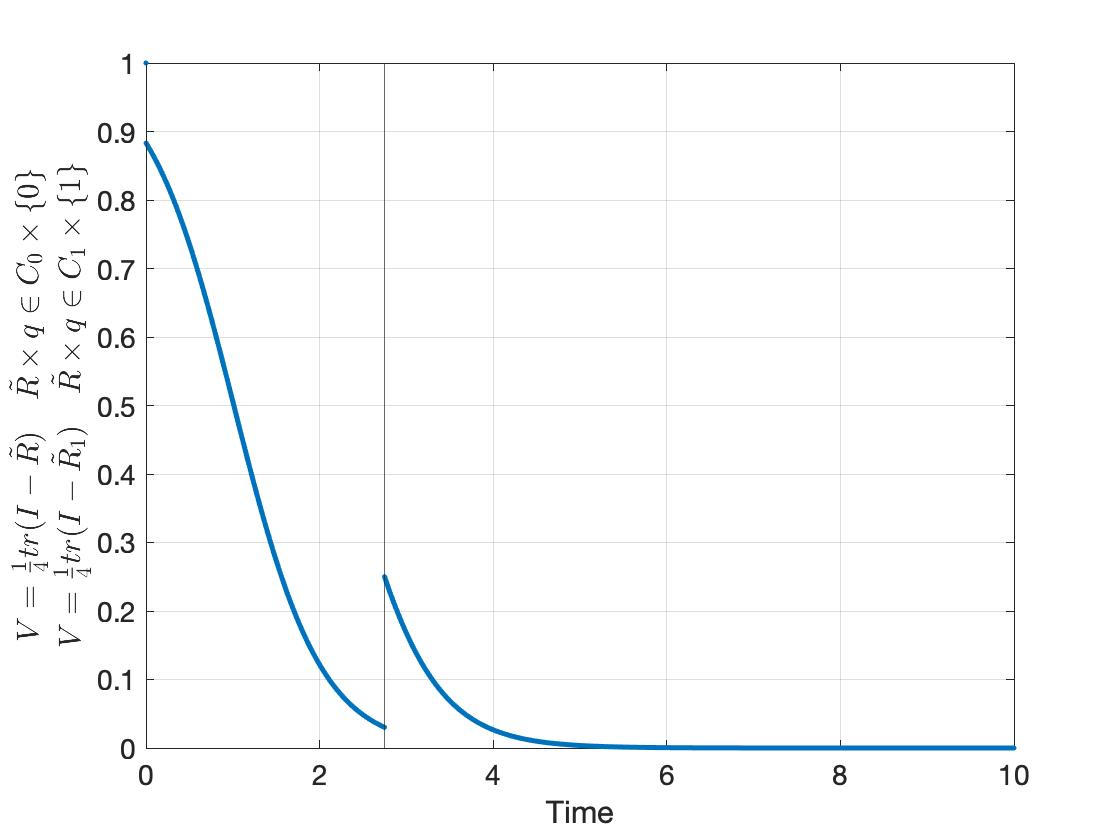
\includegraphics[width=\linewidth]{Figures/PCF_potential.jpg}
  \captionof{figure}{Plot of $V(\normSOthree{\Rtilde}, q)$ vs time.  Jumps are seen at $t_{j1}=0$ sec and $t_{j2}=2.747$ sec.}
  \label{fig:PCF_potential}
\end{minipage}\hfill
\begin{minipage}{.45\textwidth}
  \centering 
  \vspace{0pt}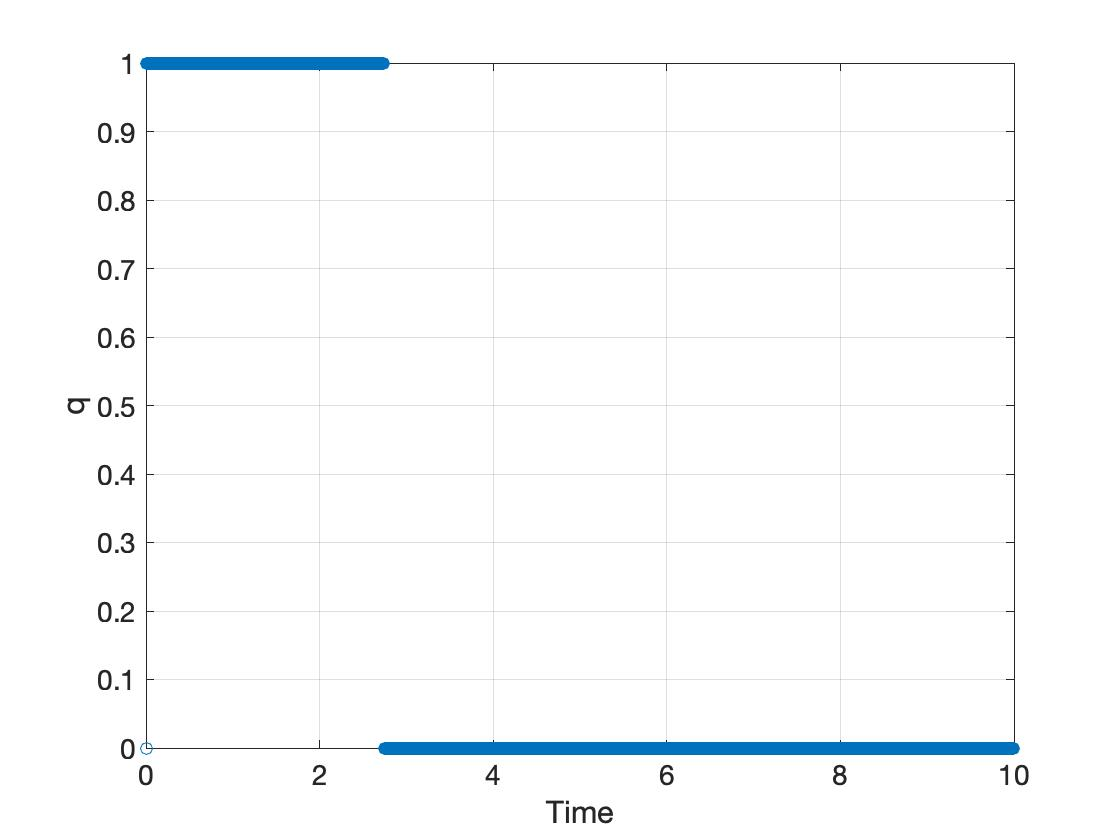
\includegraphics[width=\linewidth]{Figures/PCF_q.jpg}
  \captionof{figure}{Plot of $q(t)$ vs time.}
  \label{fig:PCF_q}
\end{minipage}
\end{figure}


\section{Hybrid Explicit Complementary Filter}

This section develops a hybrid globally exponentially stable observer derived from the explicit complementary filter presented in \cite{mahony_complementaryFilter}. Unlike the passive complementary filter, vector measurements are considered instead of measurements on $\SOthree$ which allows for an implementable version of the filter. 
The IMU sensor onboard is assumed to measure some fixed inertial directions $r_i$, where $i=1,2,..n$. This measurement of $r_i$ in the body frame is denoted by $b_i$. The true vectors and the measured vectors are related as $b_i = R^\top r_i \quad \forall i = 1,2,...,n$. To be able to extract the attitude estimate $\hat{R}$ from the measurements, we assume that $n\geq 2$ and at least two of the fixed inertial directions are noncollinear. 

% \begin{assumption}[Measurement model]
%     The measurements of fixed inertial direction $r_i$ in the body frame is given by $b_i$, $i=1,...,n$. Atleast two noncollinear fixed inertial vectors are required, $n\geq 2$. 
%     \begin{align}\label{eq:measmodel_ECF}
%         b_i = R^\top r_i \quad i=1,...,n
%     \end{align}
% \end{assumption}

Further, each of the vector measurements is assigned a weight $k_i > 0$ where $i=1,2,...n$. This allows to increase the weight of the measurement in which we have more confidence.  

\begin{assumption}\label{assumption:explicit}
The measurements are assumed to be obtained from gyroscope and IMU sensors onboard the robot. We assume the following:
\begin{enumerate}
    \item The gyroscope and IMU measurements are noise free, i.e.
    \begin{align}\label{eq:measmodel_explicit}
        \Omegay \coloneqq \Omega && b_i = R^\top r_i\quad \forall i = 1,2,..n
    \end{align}
    where $n\geq 2$, and atleast two fixed inertial vectors $r_i$ are noncollinear. 
    \item The gains $k_i$ are normalized, i.e. $\sum_{i=1}^n k_i = 1. $
\end{enumerate}
\end{assumption}

\begin{assumption}\label{assumption:distinctEigOfM0}
    Consider $M_0 \coloneqq \sum_{i=1}^n k_ir_ir_i^\top $. The gains $k_i > 0$ are chosen such that Assumption \ref{assumption:explicit} is satisfied and $M_0\coloneqq \sum_{i=1}^n k_ir_ir_i^\top $ has three distinct eigenvalues. 
\end{assumption}

\begin{lemma}\label{lemma:5}
    Given inertial directions $r_i, i=1,...,n$ and the corresponding measurements $b_i, i=1,...,n$, and the estimate $\hat{R}$ of the true attitude $R$, the left invariant estimation error is $\Rtilde\coloneqq \hat{R}^\top R$ and the right invariant estimation error is $\bar{R}\coloneqq \hat{R}R^\top $. Define $M_0 \coloneqq \sum_{i=1}^n k_i r_ir_i^\top $ and $M \coloneqq R^\top M_0R$. Then
    \begin{align}
        \trace{\bar{R}M_0} &= 1 + (1-\cos\Tilde{\theta})\trace{w_\times^2M_0}\label{eq:44}\\
        \trace{w_\times^2 M_0} &= -1 + \sum_{i=1}^n k_i (w^\top r_i)^2 \label{eq:45}
    \end{align}
    where $\Tilde{\theta}\in\R{}$ and $w\in\mathbb{S}^2$ are such that $\bar{R} = \mathcal{R}(\Tilde{\theta}, w)$. 
\end{lemma}
\begin{proof}
    We can write $\bar{R}$ using the Rodrigues rotation formula as $\bar{R} = I + w_\times\sin\Tilde{\theta} + w^2_\times (1 - \cos\Tilde{\theta})$. Now, $\trace{\bar{R}M_0} = \trace{M_0 + (1-\cos\Tilde{\theta})w^2_\times M_0}$. Since $k_i$ are normalized weights, $\trace{M_0}=1$, this proves \eqref{eq:44}. 
    Next, $\text{tr}(w_\times^2M_0) = \sum_{i=1}^n k_i \trace{w_\times^2r_ir_i^\top }$. Now, with $w = [w_1, w_2, w_3]^\top \in\mathbb{S}^1$ and $r_i =[r_{i,1}, r_{i,2}, r_{i,3}]^\top  \in\mathbb{S}^1$, we get
    \begin{align*}
        w_\times^2r_ir_i^\top  &= \begin{bmatrix}
            0 && -w_3 && w_2\\
            w_3 && 0 && -w_1\\
            -w_2 && w_1 && 0
        \end{bmatrix}\begin{bmatrix}
            r_{i,1}^2 && r_{i,1}r_{i,2} && r_{i,1}r_{i,3}\\
            r_{i,1}r_{i,2} && r_{i,2}^2 && r_{i,2}r_{i,3}\\
            r_{i,1}r_{i,3} && r_{i,2}r_{i,3} && r_{i,3}^2
        \end{bmatrix}\\
        \implies \trace{w_\times^2r_ir_i^\top } &= -1 + (w^\top r_i)
    \end{align*}
    Now, $\trace{w_\times^2M_0} = -\sum_{i=1}^n k_i + \sum_{i=1}^nk_i(w^\top r_i)^2 = -1 + \sum_{i=1}^n(w^\top r_i)^2$. This completes the proof. 
\end{proof}

Next, similar to Definition \ref{def:config_err}, we define a configuration error function in terms of vectorial measurements. 

\begin{definition}[Estimation error function]\label{def:estimationErrorFunc}
Given $n$ fixed inertial directions $r_i$, the corresponding measurements $b_i$, the corresponding relative weights as $k_i, i=1,...,n$ and the attitude estimate as $\hat{R}$, the estimation error function $\Psi:\SOthree\times \R{3\times n}\times \R{3\times n} \to \R{}$ is given below:
\begin{align}\label{eq:estimationErrorFunc}
    \Psi(\hat{R}, \{b_i\}_{i=1}^n, \{r_i\}_{i=1}^n) \coloneqq \frac{1}{4}\sum_{i=1}^n k_i \|b_i - \hat{R}^\top r_i\|^2
\end{align}
\end{definition}

\begin{lemma}\label{lemma:estErrorFunc}
    The estimation error function in \eqref{eq:estimationErrorFunc} can be simplified as follows. 
    \begin{align}
        \Psi(\hat{R}, \mathbf{b}, \mathbf{r}) = \normSOthree{\Rtilde} \left[ 1- \sum_{i=1}^n k_i(w^\top r_i)^2\right]
    \end{align}
    where $\mathbf{b}\coloneqq \{b_i\}_{i=1}^n$, $\mathbf{r}\coloneqq \{r_i\}_{i=1}^n$, and $\Tilde{\theta}\in [0,\pi]$, $v\in\R{3}$ is such that $\bar{R}\coloneqq \hat{R}R^\top  = \mathcal{R}(\Tilde{\theta}, w)$.
\end{lemma}
\begin{proof}
    For brevity, $\Psi \equiv \Psi(\hat{R}, \mathbf{b}, \mathbf{r})$. 
    \begin{align*}
        \Psi &= \frac{1}{4}\sum_{i=1}^n k_i\|b_i - \hat{R}^\top r_i\|^2\\
        &= \frac{1}{4}\sum_{i=1}^nk_i\|R^\top r_i - \hat{R}^\top r_i\|^2\\
        &= \frac{1}{2}\sum_{i=1}^n k_i \left[1 - r_i^\top \hat{R}R^\top r_i\right]\\
        &= \frac{1}{2}\sum_{i=1}^n k_i \left[1 - \trace{\hat{R}R^\top r_ir_i^\top }\right]\\
        &= \frac{1}{2}\sum_{i=1}^n \left[1 - \trace{\bar{R}M_0}\right]
        \intertext{Using Lemma \ref{lemma:5} results in the following.}
        \Psi&= \frac{1-\cos{\Tilde{\theta}}}{2}\left[ 1 - \sum_{i=1}^n k_i(w^\top r_i)^2\right] = \normSOthree{\Rtilde}\left[1 -\sum_{i=1}^nk_i(w^\top r_i)^2\right]
    \end{align*}
\end{proof}
The explicit complementary filter from \cite{mahony_complementaryFilter} is now stated below. 

\begin{theorem}[Explicit Complementary Filter {\cite[Theorem 5.1]{mahony_complementaryFilter}}]\label{theorem:explicitMahony}
Consider the system in \eqref{eq:rotationKinematics} with the measurement model in \eqref{eq:measmodel_explicit} with the observer gain $k_p > 0$, the measurement gains $k_i>0$ for $i=1,...,n$ following Assumption \ref{assumption:explicit} and Assumption \ref{assumption:distinctEigOfM0}. Consider the following filter dynamics:
\begin{alignat}{3}\label{eq:explicitMahony}
    \dot{\hat{R}} &= \hat{R}\brackets{\Omegay + k_p\omega_{mes}(\hat{R}, \mathbf{b}. \mathbf{r})}_\times, \quad \hat{R}(0) = \hat{R}_0\\
    \omega_{mes}(\hat{R}, \mathbf{b}, \mathbf{r})&\coloneqq \sum_{i=1}^n k_i \left[b_i\times (\hat{R}^\top r_i)\right],\quad k_i> 0 \text{ for } i=1,...,n
\end{alignat}
where $\mathbf{b}\coloneqq \{b_i\}_{i=1}^n$, $\mathbf{r}\coloneqq \{r_i\}_{i=1}^n$ and let $t\mapsto \hat{R}(t)$ denote the solution to \eqref{eq:explicitMahony}. Consider the left invariant estimation error $\Rtilde\coloneqq \hat{R}^TR$. Assume that $\Omega(t)$ is a bounded, absolutely continuous function and the pair $(\Omega(t), \Rtilde(t))$ are asymptotically independent. Then:
\begin{enumerate}
    \item There are three unstable equilibria of the filter characterized by
    \begin{align*}
        \hat{R}_{*i} = U_0D_iU_0^\top R, \quad i=1,2,3
    \end{align*}
    where $D_i = \texttt{diag}(1,-1,-1)$, $D_2 = \texttt{diag}(-1,1,-1)$ and $D_3=\texttt{diag}(-1,-1,1)$, and $U_0\in\SOthree$ such that $M_0 = U_0\Lambda U_0^\top $ (where $M_0$ is defined in Assumption \ref{assumption:distinctEigOfM0}) and $\Lambda = \texttt{diag}(\lambda_1, \lambda_2, \lambda_3)$ is the diagonal matrix of distinct eigenvalues of $M_0$. \label{item:a-mahony-ecf}
    \item The set $\{I\}$ is locally exponentially stable for $\Rtilde$ dynamics. \label{item:b-mahony-ecf}
    \item For almost all initial conditions $\Tilde{R}_0\neq \hat{R}^\top _{*i}R(0), i=1,2,3$, $\hat{R}(t)$ converges to $R(t)$, and for each positive $k$ such that $0 < k < 1-\xi$ where $\xi \coloneqq \max_{u\in\mathbb{S}^2}\sum_{i=1}^n k_i(u^Tr_i)^2$ and $\normSOthree{\Rtilde^y(0)}\leq k$, every solution $t\mapsto \Rtilde(t)$ to the observer error dynamics satisfies \label{item:c-mahony-ecf}
    \begin{align} \label{eq:localExpStability_ECF}
    \normSOthree{\Rtilde(t)}\leq \expo{-k_p(1-\xi)(1-k)t}\normSOthree{\Rtilde(0)}\quad \forall t\in\dom\Rtilde.
\end{align}
\end{enumerate}
\end{theorem}
\begin{proof}
    See \cite[Theorem 5.1]{mahony_complementaryFilter} for the proof of \ref{item:a-mahony-ecf}, \ref{item:b-mahony-ecf}. For the proof of \ref{item:c-mahony-ecf}, consider the Lyapunov function candidate $V(\Rtilde) = \normSOthree{\Rtilde}$. Note that this Lyapunov function candidate is different from the one used in \cite[Theorem 5.1]{mahony_complementaryFilter}. The derivative of $V$ along the trajectory of $\Rtilde$ gives
     \begin{align*}
         \dualpairing{\grad{\Rtilde}{V}}{\dot{\Rtilde}} &= -\frac{1}{4}\trace{\dot\Rtilde}\\
         &= \frac{k_p}{4}\trace{\omega_{mes}(\hat{R}, \mathbf{b}, \mathbf{r})_\times \mathbb{P}_a(\Rtilde)}\\
         &= \frac{k_p}{4}\trace{\mathbb{P}_a(\Rtilde M)\mathbb{P}_a(\Rtilde)}
         \intertext{where $M = R^\top M_0R$.}
         \dualpairing{\grad{\Rtilde}{V}}{\dot{\Rtilde}}  &= \frac{k_p}{8}\trace{\Rtilde^2M - M}\\
         \intertext{Now, with $\Rtilde = \mathcal{R}(\Tilde{\theta}, x)$ for some $\Tilde{\theta}\in \R{}$ and $x\in\mathbb{S}^2$, using $\Rtilde^2 = I + x_\times \sin\Tilde{\theta} + x_\times^2 (1-\cos\Tilde{\theta})$ results in}
         \dualpairing{\grad{\Rtilde}{V}}{\dot{\Rtilde}}  &=\frac{k_p}{4}\normSOthree{\Rtilde^2}\trace{x_\times^2R^\top M_0R}\\
         &= \frac{k_p}{4}\trace{w_\times^2 M_0}\\
         \intertext{where $w\coloneqq Rx$. Now using Lemma \ref{lemma:5} results in the following.}
         \dualpairing{\grad{\Rtilde}{V}}{\dot{\Rtilde}} &= -\frac{k_p}{4}\normSOthree{\Rtilde^2}\left[1 - \sum_{i=1}^n k_i(w^\top r_i)^2\right]\\
         &\leq -k_p\normSOthree{\Rtilde}(1-k)(1-\xi)\\
         \implies \normSOthree{\Rtilde(t)}&\leq \expo{-k_p(1-\xi)(1-k)t}\normSOthree{\Rtilde(0)} \quad \forall t\in \dom\Rtilde. 
     \end{align*}
\end{proof}

\begin{remark}\label{remark:explicitFilter_unstable}
    Note that in Theorem \ref{theorem:explicitMahony}, $U_0D_iU_0^\top $ represents a rotation of $180^\circ$ about the axis given by $U_0e_i$ where $e_i$ is the standard basis vector. Thus, the unstable equilibria of the explicit complementary filter are when the right invariant estimation error ($\bar{R}\coloneqq \hat{R}R^\top $) represents a $180^\circ$ rotation about the axis of rotation given by either $U_0e_1$, $U_0e_2$ or $U_0e_3$. This is unlike the passive complementary filter in Theorem \ref{thm:mahony} which is unstable for $180^\circ$ observer error about any axis of rotation. 
\end{remark}

% \begin{lemma}\label{lemma:5}
%     Given inertial directions $r_i, i=1,...,n$ and the corresponding measurements $b_i, i=1,...,n$, and the estimate $\hat{R}$ of the true attitude $R$, the left invariant estimation error is $\Rtilde\coloneqq \hat{R}^\top R$ and the right invariant estimation error is $\bar{R}\coloneqq \hat{R}R^\top $. Define $M_0 \coloneqq \sum_{i=1}^n k_i r_ir_i^\top $ and $M \coloneqq R^\top M_0R$. Then
%     \begin{align}
%         \trace{\bar{R}M_0} &= 1 + (1-\cos\Tilde{\theta})\trace{w_\times^2M_0}\label{eq:44}\\
%         \trace{w_\times^2 M_0} &= -1 + \sum_{i=1}^n k_i (w^\top r_i)^2 \label{eq:45}
%     \end{align}
%     where $\Tilde{\theta}\in\R{}$ and $w\in\mathbb{S}^2$ are such that $\bar{R} = \mathcal{R}(\Tilde{\theta}, w)$. 
% \end{lemma}
% \begin{proof}
%     We can write $\bar{R}$ using the Rodrigues rotation formula as $\bar{R} = I + w_\times\sin\Tilde{\theta} + w^2_\times (1 - \cos\Tilde{\theta})$. Now, $\trace{\bar{R}M_0} = \trace{M_0 + (1-\cos\Tilde{\theta})w^2_\times M_0}$. Since $k_i$ are normalized weights, $\trace{M_0}=1$, this proves \eqref{eq:44}. 
%     Next, $\text{tr}(w_\times^2M_0) = \sum_{i=1}^n k_i \trace{w_\times^2r_ir_i^\top }$. Now, with $w = [w_1, w_2, w_3]^\top \in\mathbb{S}^1$ and $r_i =[r_{i,1}, r_{i,2}, r_{i,3}]^\top  \in\mathbb{S}^1$, we get
%     \begin{align*}
%         w_\times^2r_ir_i^\top  &= \begin{bmatrix}
%             0 && -w_3 && w_2\\
%             w_3 && 0 && -w_1\\
%             -w_2 && w_1 && 0
%         \end{bmatrix}\begin{bmatrix}
%             r_{i,1}^2 && r_{i,1}r_{i,2} && r_{i,1}r_{i,3}\\
%             r_{i,1}r_{i,2} && r_{i,2}^2 && r_{i,2}r_{i,3}\\
%             r_{i,1}r_{i,3} && r_{i,2}r_{i,3} && r_{i,3}^2
%         \end{bmatrix}\\
%         \implies \trace{w_\times^2r_ir_i^\top } &= -1 + (w^\top r_i)
%     \end{align*}
%     Now, $\trace{w_\times^2M_0} = -\sum_{i=1}^n k_i + \sum_{i=1}^nk_i(w^\top r_i)^2 = -1 + \sum_{i=1}^n(w^\top r_i)^2$. This completes the proof. 
% \end{proof}

% Next, similar to Definition \ref{def:config_err}, we define a configuration error function in terms of vectorial measurements. 

% \begin{definition}[Estimation error function]\label{def:estimationErrorFunc}
% Given $n$ fixed inertial directions $r_i$, the corresponding measurements $b_i$, the corresponding relative weights as $k_i, i=1,...,n$ and the attitude estimate as $\hat{R}$, the estimation error function $\Psi:\SOthree\times \R{3\times n}\times \R{3\times n} \to \R{}$ is given below:
% \begin{align}\label{eq:estimationErrorFunc}
%     \Psi(\hat{R}, \{b_i\}_{i=1}^n, \{r_i\}_{i=1}^n) \coloneqq \frac{1}{4}\sum_{i=1}^n k_i \|b_i - \hat{R}^\top r_i\|^2
% \end{align}
% \end{definition}

% \begin{lemma}\label{lemma:estErrorFunc}
%     The estimation error function in \eqref{eq:estimationErrorFunc} can be simplified as follows. 
%     \begin{align}
%         \Psi(\hat{R}, \mathbf{b}, \mathbf{r}) = \normSOthree{\Rtilde} \left[ 1- \sum_{i=1}^n k_i(w^\top r_i)^2\right]
%     \end{align}
%     where $\mathbf{b}\coloneqq \{b_i\}_{i=1}^n$, $\mathbf{r}\coloneqq \{r_i\}_{i=1}^n$, and $\Tilde{\theta}\in [0,\pi]$, $v\in\R{3}$ is such that $\bar{R}\coloneqq \hat{R}R^\top  = \mathcal{R}(\Tilde{\theta}, w)$.
% \end{lemma}
% \begin{proof}
%     For brevity, $\Psi \equiv \Psi(\hat{R}, \mathbf{b}, \mathbf{r})$. 
%     \begin{align*}
%         \Psi &= \frac{1}{4}\sum_{i=1}^n k_i\|b_i - \hat{R}^\top r_i\|^2\\
%         &= \frac{1}{4}\sum_{i=1}^nk_i\|R^\top r_i - \hat{R}^\top r_i\|^2\\
%         &= \frac{1}{2}\sum_{i=1}^n k_i \left[1 - r_i^\top \hat{R}R^\top r_i\right]\\
%         &= \frac{1}{2}\sum_{i=1}^n k_i \left[1 - \trace{\hat{R}R^\top r_ir_i^\top }\right]\\
%         &= \frac{1}{2}\sum_{i=1}^n \left[1 - \trace{\bar{R}M_0}\right]
%         \intertext{Using Lemma \ref{lemma:5} results in the following.}
%         \Psi&= \frac{1-\cos{\Tilde{\theta}}}{2}\left[ 1 - \sum_{i=1}^n k_i(w^\top r_i)^2\right] = \normSOthree{\Rtilde}\left[1 -\sum_{i=1}^nk_i(w^\top r_i)^2\right]
%     \end{align*}
% \end{proof}

%  \begin{lemma}\label{lemma:localExpStability_ECF}
% Consider the system \eqref{eq:rotationKinematics} with an absolutely continuous and bounded $t\mapsto \Omega(t)$ and the observer in Theorem \ref{theorem:explicitMahony} with initial condition such that $\normSOthree{\Rtilde(0)} \neq 1$. With $\xi\coloneqq \max_{u\in\mathbb{S}^2}\sum_{i=1}^nk_i(u^\top r_i)^2$, there exists $k>0$ such that $\normSOthree{\Rtilde(0)} \leq k < 1-\xi$ and every solution $t\mapsto \Rtilde(t)$ to the error dynamics satisfies
% \begin{align}
%     \normSOthree{\Rtilde(t)}\leq \expo{-k_p(1-\xi)(1-k)t}\normSOthree{\Rtilde(0)}\quad \forall t\in\dom\Rtilde.
% \end{align}
%  \end{lemma}
%  \begin{proof}
%      Consider the Lyapunov function candidate $V(\Rtilde) = \normSOthree{\Rtilde}$. Note that this Lyapunov function candidate is different from the one used in \cite{mahony_complementaryFilter}. The derivative of $V$ along the trajectory of $\Rtilde$ gives
%      \begin{align*}
%          \dualpairing{\grad{\Rtilde}{V}}{\dot{\Rtilde}} &= -\frac{1}{4}\trace{\dot\Rtilde}\\
%          &= \frac{k_p}{4}\trace{\omega_{mes}(\hat{R}, \mathbf{b}, \mathbf{r})_\times \mathbb{P}_a(\Rtilde)}\\
%          &= \frac{k_p}{4}\trace{\mathbb{P}_a(\Rtilde M)\mathbb{P}_a(\Rtilde)}
%          \intertext{where $M = R^\top M_0R$.}
%          \dualpairing{\grad{\Rtilde}{V}}{\dot{\Rtilde}}  &= \frac{k_p}{8}\trace{\Rtilde^2M - M}\\
%          \intertext{Now, with $\Rtilde = \mathcal{R}(\Tilde{\theta}, x)$ for some $\Tilde{\theta}\in \R{}$ and $x\in\mathbb{S}^2$, using $\Rtilde^2 = I + x_\times \sin\Tilde{\theta} + x_\times^2 (1-\cos\Tilde{\theta})$ results in}
%          \dualpairing{\grad{\Rtilde}{V}}{\dot{\Rtilde}}  &=\frac{k_p}{4}\normSOthree{\Rtilde^2}\trace{x_\times^2R^\top M_0R}\\
%          &= \frac{k_p}{4}\trace{w_\times^2 M_0}\\
%          \intertext{where $w\coloneqq Rx$. Now using Lemma \ref{lemma:5} results in the following.}
%          \dualpairing{\grad{\Rtilde}{V}}{\dot{\Rtilde}} &= -\frac{k_p}{4}\normSOthree{\Rtilde^2}\left[1 - \sum_{i=1}^n k_i(w^\top r_i)^2\right]\\
%          &\leq -k_p\normSOthree{\Rtilde}(1-k)(1-\xi)\\
%          \implies \normSOthree{\Rtilde(t)}&\leq \expo{-k_p(1-\xi)(1-k)t}\normSOthree{\Rtilde(0)} \quad \forall t\geq 0
%      \end{align*}
%  \end{proof}

\section{Hybrid explicit complementary filter}
In this section, we extend the explicit complementary filter in Theorem \ref{theorem:explicitMahony} to obtain a globally convergent observer. Next, similar to \eqref{eq:unstable_observer}, we define a rotated observer below. 
\begin{subequations}\label{eq:unstable_observer_explicit}
\begin{align}
    \dot{\hat{R}} &= \hat{R}\brackets{\Omegay + \overline{k_p}\omega_{mes}(\hat{R}, \mathbf{b}, {R^{*}}^\top \mathbf{r})}_\times,\quad \hat{R}(0) = \hat{R}_0, \quad\overline{k_p}>0\\
    \omega_{mes}(\hat{R}, \mathbf{b}, {R^*}^\top \mathbf{r})&\coloneqq \sum_{i=1}^n \overline{k_i} \left[b_i\times (\hat{R}^\top {R^*}^\top r_i)\right],\quad \overline{k_i}> 0, \quad i=1,..., n
\end{align}
\end{subequations}
where $\mathbf{b}\coloneqq \{b_i\}_{i=1}^n$ and $\mathbf{r}\coloneqq \{r_i\}_{i=1}^n$. It is straightforward from Theorem \ref{theorem:explicitMahony} to see that \eqref{eq:unstable_observer_explicit} ensures that $R^*$ is a locally exponentially stable equilibrium point of the right invariant observer error ($\bar{R}$) dynamics. We now move towards deriving the hybrid explicit complementary filter.  


Let $\xi = \max_{u\in\mathbb{S}^2} \sum_{i=1}^nk_i (u^\top r_i)^2$. Define positive constants $c_0, c_1$ such that $0 < c_1 < c_0 < 1-\xi$. For the hybrid observer, we define the flow and jump sets below. 

% \begin{subequations}
% \begin{align}
%     C_0 \coloneqq \{(\hat{R}, \mathbf{b}, \mathbf{r})\in\SOthree\times \R{3\times n}\times \R{3\times n}\mid \Psi(\hat{R}, \mathbf{b}, \mathbf{r}) \leq c_0\}\\
%     D_0 \coloneqq \{(\hat{R}, \mathbf{b}, \mathbf{r})\in\SOthree\times \R{3\times n}\times \R{3\times n}\mid \Psi(\hat{R}, \mathbf{b}, \mathbf{r}) \geq c_0\}\\
%     C_1 \coloneqq \{(\hat{R}, \mathbf{b}, \mathbf{r})\in\SOthree\times \R{3\times n}\times \R{3\times n}\mid \Psi(\hat{R}, \mathbf{b}, \mathbf{r}) \geq c_1\}\\
%     D_1 \coloneqq \{(\hat{R}, \mathbf{b}, \mathbf{r})\in\SOthree\times \R{3\times n}\times \R{3\times n}\mid \Psi(\hat{R}, \mathbf{b}, \mathbf{r}) \leq c_1\}
% \end{align}
% \end{subequations}

\begin{subequations}
\begin{align}
    C_0 \coloneqq {\{(\hat{R}, \mathbf{b}, \mathbf{r})\in\SOthree\times \R{3\times n}\times \R{3\times n}\mid \Psi(\hat{R}, \mathbf{b}, \mathbf{r}) \leq c_0 \}}\\
    D_0 \coloneqq {\{(\hat{R}, \mathbf{b}, \mathbf{r})\in\SOthree\times \R{3\times n}\times \R{3\times n}\mid \Psi(\hat{R}, \mathbf{b}, \mathbf{r}) \geq c_0 \}}\\
    C_1 \coloneqq {\{(\hat{R}, \mathbf{b}, \mathbf{r})\in\SOthree\times \R{3\times n}\times \R{3\times n}\mid \Psi(\hat{R}, \mathbf{b}, \mathbf{r}) \geq c_1 \}}\\
    D_1 \coloneqq {\{(\hat{R}, \mathbf{b}, \mathbf{r})\in\SOthree\times \R{3\times n}\times \R{3\times n}\mid \Psi(\hat{R}, \mathbf{b}, \mathbf{r}) \leq c_1\}}
\end{align}
\end{subequations}
The state of the hybrid observer, denoted by $\hat{\mathcal{H}}_2$, is $q\in Q\coloneqq \{0, 1\}$, the input is $v \coloneqq (\hat{R}, \mathbf{b}, \mathbf{r}, \Omegay)\in \SOthree\times \R{3\times n}\times \R{3\times n} \times \R{}$ and the output $\zeta=f(q,v)\coloneqq (f_1(q,v), f_2(q,v))\in\sothree\times Q$ is defined in \eqref{eq:hybrid-observer-ecf-output}. Define $\gamma_i(v) \coloneqq (\Omegay + k_i\omega_i)_\times$, $i=1,2$ where $\omega_0 \coloneqq \omega_{mes}(\hat{R}, \mathbf{b}, \mathbf{r})$, $\omega_1 \coloneqq \omega_{mes}(\hat{R}, \mathbf{b}, \Rstar^\top\mathbf{r})$ and $k_0 \coloneqq k_p$, $k_1\coloneqq \overline{k_p}$. The data for the hybrid observer $\hat{\mathcal{H}}_2 = ({\hat{C}, \hat{F}, \hat{D}, \hat{G}, \zeta})$ is given as 


% The hybrid observer $\hat{H}_2$ can be represented by the states $q\in Q\coloneqq\{0,1\}$. The inputs for $\hat{H}_2$ are $u \coloneqq (\hat{R}, \mathbf{b}, \mathbf{r}, \Omegay)\in\SOthree\times\R{3\times n}\times \R{3\times n}\times \R{3}$, the output $\zeta: \SOthree\times\R{3\times n}\times \R{3\times n}\times \R{3}\times Q\to\sothree$ is defined below. Define $\gamma_i(u) = \brackets{\Omegay + k_p\omega_i}_\times, \:i=0,1$ where $\omega_0 \coloneqq \omega_{mes}(\hat{R}, \mathbf{b}, \mathbf{r})$ and $\omega_1 \coloneqq \omega_{mes}(\hat{R}, \mathbf{b}, {\Rstar}^\top \mathbf{r})$. The data for the hybrid observer $\hat{H}_2 = (C_K, F_K, D_K, G_K, \zeta)$ is given as follows.  
% \begin{align}
%     C_K &= \bigcup_{q\in Q}\brackets{C_{K, q}\times q}, \quad \begin{cases}
%         C_{K, 0} \coloneqq C_0\\
%         C_{K, 1} \coloneqq C_1
%     \end{cases}\\
%     F_K(u, q) &= 0\\
%     D_K &= \bigcup_{q\in Q} \brackets{D_{K, q}\times Q}, \quad \begin{cases}
%         D_{K,0} \coloneqq D_0\\
%         D_{K,1} \coloneqq D_1
%     \end{cases}\\
%     G_K(u, q) &= 1 - q \\
%     \zeta(u, q) &= q\gamma_1(u) + (1-q)\gamma_0(u)
% \end{align}

\begin{subequations}
\begin{align}
    \hat{C} &= \bigcup_{q\in Q}\brackets{\hat{C}_{q}\times q}, \quad \begin{cases}
        \hat{C}_{0} \coloneqq C_0\\
        \hat{C}_{1} \coloneqq C_1
    \end{cases}\\
    \hat{F}(q, v) &= 0\\
    \hat{D} &= \bigcup_{q\in Q} \brackets{\hat{D}_{q}\times q}, \quad \begin{cases}
        \hat{D}_{0} \coloneqq D_0\\
        \hat{D}_{1} \coloneqq D_1
    \end{cases}\\
    \hat{G}(q, v) &= 1 - q \\
    \zeta &= f(q,v)\coloneqq (\underbrace{q\gamma_1(v) + (1-q)\gamma_0(v)}_\text{$f_1(q, v)$}, \underbrace{q}_\text{$f_2(q,v)$}) \label{eq:hybrid-observer-ecf-output}
\end{align}
\end{subequations}
Using the above hybrid observer, the estimates are updated as 
\begin{align}\label{eq:hybrid_observer_ECF}
\underbrace{\dot{\hat{R}} = \hat{R}f_1(q, v), \quad \dot{q} = 0}_{\text{during flows}}, \quad \text{ and}\quad \quad   \underbrace{\hat{R}^+ = \hat{R}, \quad q^+ = 1 - q}_\text{during jumps}
\end{align}

Consider the hybrid system $\mathcal{H}_2 = (C, F, G, D)$, that represents the observer error, with the states $\eta \coloneqq (\Rtilde, q) \in \SOthree\times Q$ and inputs $\rho \coloneqq (\hat{R}, \mathbf{b}, \mathbf{r}, \Omegay, \Omega)\in\SOthree\times\R{3\times n}\times\R{3\times n}\times \R{3}\times \R{3}$ has the following data. 
\begin{subequations}\label{eq:hybrid_observer_error_explicit}
\begin{align}
C&\coloneqq \hat{C}\\
F(\eta, \rho)&\coloneqq \begin{bmatrix}
    \Rtilde\brackets{\Rtilde^\top f_1(q, v)^\top \Rtilde + \Omega_\times}\\ 0\end{bmatrix} \label{eq:Rtilde_dot_ecf}\\
D &\coloneqq \hat{D}\\
G(\eta, \rho) &\coloneqq \begin{bmatrix}
\Rtilde \\ 1 - q
\end{bmatrix}
\end{align}
\end{subequations}
where $v = (\hat{R}, \mathbf{b}, \mathbf{r}, \Omegay)$ and \eqref{eq:Rtilde_dot_ecf} is obtained by substituting $\dot{\hat{R}}$ from \eqref{eq:hybrid_observer_ECF} in $\dot{\Rtilde} = \dot{\hat{R}}^\top R + \hat{R}^\top \dot{R}$. 


% Consider the hybrid system $\mathcal{H}_2 = (C, F, G, D)$ that represents the observer error with the states $(\Rtilde, q) \in \SOthree\times Q$, inputs $()$ and has the following data. 
% \begin{subequations}\label{eq:hybrid_observer_error_explicit}
% \begin{align}
% C&\coloneqq C_K\\
% F(\Rtilde, q)&\coloneqq \begin{bmatrix}
%     \Rtilde\brackets{\Rtilde^\top \zeta(u, q)^\top \Rtilde + \Omega_\times}\\ 0\end{bmatrix}\\
% D &\coloneqq D_K\\
% G(\Rtilde, q) &\coloneqq \begin{bmatrix}
% \Rtilde \\ 1 - q
% \end{bmatrix}
% \end{align}
% \end{subequations}

% \begin{theorem}[Hybrid explicit complementary filter]\label{theorem:hybridECF}
% Given the system \eqref{eq:rotationKinematics} and consider the set $\mathcal{A}\coloneqq \{I\}\times \{0\}\in\SOthree\times Q$. Define $\xi\coloneqq \max_{u\in\mathbb{S}^2}\sum_{i=1}^nk_i(u^\top r_i)^2$. If there exist constants $c_0, c_1, d_0, e_0, f_0 > 0$ and $\Rstar\in\SOthree$ such that the following holds:

% \begin{enumerate}[(a)]
%         \item $0 < e_0 < f_0 < c_1 < c_0 < 1-\xi$,\label{item:a-bullet-ecf}\\
%         \item $2e_0\left[1 + \sqrt{\brackets{\frac{1}{c_1}-1}\brackets{\frac{1}{f_0}-1}}\right] < 1$,
%         % \begin{align*}
%         %     2e_0\left[1 + \sqrt{\brackets{\frac{1}{c_1}-1}\brackets{\frac{1}{f_0}-1}}\right] < 1,
%         % \end{align*}
%         \item $e_0 < \normSOthree{R^*} < f_0$, \label{item:c-bullet-ecf}
%         \item {${v}^\top \hat{R}(0,0)x\neq 0$ where $x$ and $v$ are the axis of rotation of $\Rtilde^y(0,0)$ and $R^*$ respectively}, \label{item:d-bullet-ecf}
%         \item $1 - \normSOthree{\Rstar} < d_0 < 1$, \label{item:e-bullet-ecf}
% \end{enumerate}
% then:
% \begingroup
%     \renewcommand\labelenumi{(\theenumi)}
%     \begin{enumerate}
%         \item \label{(1ecf)}The hybrid observer error system $\mathcal{H}_2 = (C, F, D, G)$ with data given in \eqref{eq:hybrid_observer_error_explicit} satisfies the hybrid basic conditions.
%         \item \label{(2ecf)}Every maximal solution to $\mathcal{H}_2$ from $C\cup D$ is complete.
%         \item \label{(3ecf)} Every maximal solution to $\mathcal{H}_2$ exhibits no more than 2 jumps. 
%         \item \label{(4ecf)}The set $\mathcal{A}$ is globally exponentially stable for $\mathcal{H}_2$. 
%     \end{enumerate}
%     \endgroup
% \end{theorem}




\begin{theorem}[Hybrid explicit complementary filter]\label{theorem:hybridECF}
Given the system \eqref{eq:rotationKinematics} and consider the set $\mathcal{A}\coloneqq \{I\}\times \{0\}\in\SOthree\times Q$. Define $\xi\coloneqq \max_{u\in\mathbb{S}^2}\sum_{i=1}^nk_i(u^\top r_i)^2$. Assume that $\Omega(t)$ is a bounded and absolutely continuous. If there exist constants $k_p, \overline{k_p}, c_0, c_1 > 0$ and $\Rstar\in\SOthree$ such that

\begin{enumerate}[(a)]
        \item $0 < \normSOthree{\Rstar} < c_1 < c_0 < 1-\xi$,\label{item:a-bullet-ecf}\\
        % \item $2e_0\left[1 + \sqrt{\brackets{\frac{1}{c_1}-1}\brackets{\frac{1}{f_0}-1}}\right] < 1$,
        % \begin{align*}
        %     2e_0\left[1 + \sqrt{\brackets{\frac{1}{c_1}-1}\brackets{\frac{1}{f_0}-1}}\right] < 1,
        % \end{align*}
        % \item $e_0 < \normSOthree{R^*} < f_0$, \label{item:c-bullet-ecf}
        \item {${v}^\top \hat{R}(0,0)x\neq 0$ where $x$ and $v$ are the axis of rotation of $\Rtilde^y(0,0)$ and $R^*$ respectively}, \label{item:b-bullet-ecf}
        % \item $1 - \normSOthree{\Rstar} < d_0 < 1$, \label{item:e-bullet-ecf}
\end{enumerate}
then
\begingroup
    \renewcommand\labelenumi{(\theenumi)}
    \begin{enumerate}
        \item \label{(1ecf)}The hybrid observer error system $\mathcal{H}_2 = (C, F, D, G)$ with data given in \eqref{eq:hybrid_observer_error_explicit} satisfies the hybrid basic conditions.
        \item \label{(2ecf)}Every maximal solution to $\mathcal{H}_2$ from $C\cup D$ is complete.
        \item \label{(3ecf)} Every maximal solution to $\mathcal{H}_2$ exhibits no more than 2 jumps. 
        \item \label{(4ecf)}The set $\mathcal{A}$ is globally exponentially stable for $\mathcal{H}_2$. 
    \end{enumerate}
    \endgroup
\end{theorem}



\begin{proof}
The proof follows in the same manner as the proof of Theorem \ref{theorem:main}. The only difference is in the exponential bounds that we obtain. We now calculate just the bounds since the rest of it follows directly from Theorem \ref{theorem:main}. 
Due to the construction of the set $C_0$,  ${(\hat{R}(0,0), \mathbf{b}, \mathbf{r})}\in C_0 \implies \Psi(\hat{R}(0,0), \mathbf{b}, \mathbf{r}) {\leq c_0}$. Using \ref{lemma:estErrorFunc}, we have that $\Psi(\hat{R}, \mathbf{b}, \mathbf{r})\leq c_0\implies \normSOthree{\Rtilde} \leq \frac{c_0}{1-\xi}$. Now, using \eqref{eq:localExpStability_ECF}, we obtain the exponential bound when ${(\hat{R}(0,0), \mathbf{b}, \mathbf{r}, q(0,0))}\in C_0\times\{0\}$ as below. 
\begin{align}
    \normSOthree{\Rtilde(t,0)} &\leq \expo{-k_p(1-\xi-c_0)t}\normSOthree{\Rtilde(0,0)} \quad \forall t\in\dom\Rtilde.
    \intertext{Similarly, when ${(\hat{R}(0,0), \mathbf{b}, \mathbf{r}, q(0,0))}\in C_1\times\{1\}$ and using the fact that there exists $d_0$ such that $1-\normSOthree{\Rstar} < d_0 < 1$, we have }
    \normSOthree{\Rtilde_1(t,0)}&\leq \expo{-\overline{k_p}(1-\xi-d_0)t}\normSOthree{\Rtilde_1(0,0)}\quad \forall t\in\dom\Rtilde_1 \label{eq:non_rot_ecf}\\
    \intertext{Now, due to \ref{item:a-bullet-ecf}, there exist positive constants $e_0, f_0$ such that $e_0 < \normSOthree{\Rstar} < f_0 < c_1$. Using \eqref{eq:R1tilde_upperbound} and \eqref{eq:R1tilde_lowerbound}, we obtain the following. }
    \implies \normSOthree{\Rtilde(t,0)} &\leq \alpha \expo{-\overline{k_p}(1-\xi-d_0)t}\normSOthree{\Rtilde(0,0)} \quad \forall t\in\dom\Rtilde \label{eq:rot_ecf}
    \intertext{where $\alpha$ is defined in \eqref{eq:C1bounds}. Since $V(\Rtilde) = \normSOthree{\Rtilde}$ is always decreasing, there exists $T > 0$ such that ${(\hat{R}(0,0), \mathbf{b},\mathbf{r}, q(0,0))} \in C_1\times\{1\}$ which implies that ${(\hat{R}(T,0), \mathbf{b}, \mathbf{r}, q(T,0))}\in D_1\times\{1\}$, resulting in ${(\hat{R}(T,1), \mathbf{b}, \mathbf{r}, q(T,1))} \in C_0\times\{0\}$. Combining \eqref{eq:non_rot_ecf} and \eqref{eq:rot_ecf} results in}
    \normSOthree{\Rtilde(t,0)} &\leq \min\{1, \alpha \expo{-\min\{\overline{k_p}(1-d_0), k_p(1-c_0)\}t}\normSOthree{\Rtilde(0,0)}\} \quad \forall t\in \dom\Rtilde
\end{align}
Following similar arguments as the proof of Theorem \ref{theorem:main} completes the proof. 
\end{proof}

\subsection{Robustness analysis of the hybrid explicit complementary filter}
We consider measurement noise in gyro measurements $\Omegay$ as well as the vectorial direction measurements $\{b_i\}_{i=1}^n$. Consider the following measurement model
\begin{align}\label{eq:hybridECF_ISS}
    \Omegay = \Omega + \noisegyro && b_i = R^\top r_i + \noisevec_i, \quad i=1,...,n
\end{align}
with the bounds on the noise as given by $\textblue{\maxnoisegyro\coloneqq \sup_{t\geq 0}\|\noisegyro(t)\|}$ and $\textblue{\maxnoisevec \coloneqq \max_{i}\{\sup_{t\geq 0}\|\noisevec_i(t)\|\}_{i=1}^n}$. 

\begin{theorem}
    Assuming the conditions \ref{item:a-bullet}-\ref{item:b-bullet} in Theorem \ref{theorem:hybridECF} hold and $\frac{\maxnoisevec \kappa}{4} + \frac{\maxnoisegyro\kappa_\omega}{4} < 1$, where $\kappa\coloneqq \frac{1}{1-\xi-d_0} + \frac{1}{1-\xi-c_0}$ and $\kappa_\omega\coloneqq \frac{1}{\overline{k_p}(1-\xi-d_0)} + \frac{1}{k_p(1-\xi-c_0)}$. Consider the set $\A$ defined in Theorem \ref{theorem:hybridECF}. Then, the hybrid observer defined in \eqref{eq:hybrid_observer_ECF} renders the resulting observer error dynamics eventually input-to-state stable with respect to $\A$ to noisy gyroscope and direction measurements of the form presented in \eqref{eq:hybridECF_ISS}.
\end{theorem}
\begin{proof}
    Consider the case when ${(\hat{R}(0,0), \mathbf{b}, \mathbf{r}, q(0,0))} \in C_0 \times\{0\}$. This implies that $\Psi(\hat{R}(0,0), \mathbf{b}, \mathbf{r})\leq c_0$. It follows from Lemma \ref{lemma:estErrorFunc} that $\normSOthree{\Rtilde(0,0)}\leq \frac{c_0}{1-\xi}$. This case employs the observer in \eqref{eq:explicitMahony}. Consider the Lyapunov function candidate $V(\Rtilde) = \normSOthree{\Rtilde}$. The derivative of the Lyapunov function candidate along the trajectories of $\Rtilde$ is given below. 
    \begin{align}
        \dualpairing{\grad{\Rtilde}{V}}{\dot{\Rtilde}} &= -\frac{1}{4}\trace{\dot{\Rtilde}}\\
        &= \frac{k_p}{4}\trace{\omega_{mes}(\hat{R}, \mathbf{b}, \mathbf{r})_\times \Rtilde} + \frac{k_p}{4}\trace{\left[\sum_{i=1}^n k_i (\eta_i\times \hat{R}^\top r_i)\right]_\times \Rtilde} + \frac{1}{4}\trace{{\noisegyro}_\times \Rtilde} \nonumber\\
        &\leq \frac{k_p}{4}\normSOthree{\Rtilde^2}\trace{v_\times^2R^\top M_0R} + \frac{k_p}{4}\maxnoisevec + \frac{1}{4}\maxnoisegyro
        \intertext{Following the proof of \ref{eq:localExpStability_ECF}, we obtain the following.}
        \dualpairing{\grad{\Rtilde}{V}}{\dot{\Rtilde}}&\leq -k_p(1-\xi-c_0)\normSOthree{\Rtilde} + \frac{k_p}{4}\maxnoisevec + \frac{1}{4}\maxnoisegyro\nonumber\\
        \normSOthree{\Rtilde(t,0)}&\leq \expo{-k_p(1-\xi-c_0)t}\normSOthree{\Rtilde(0,0)} + \frac{\maxnoisevec}{4(1-\xi-c_0)} + \frac{\maxnoisegyro}{4k_p(1-\xi-c_0)}  \quad \forall t\in\dom\Rtilde\label{eq:ECF_ISS_C0}
        \intertext{Considering the other case when ${(\hat{R}(0,0), \mathbf{b}, \mathbf{r}, q(0,0))}\in C_1\times\{1\}$ results in the following bound. }
        \normSOthree{\Rtilde_1(t,0)} &\leq \expo{-k_p(1-\xi-d_0)t}\normSOthree{{\Rtilde_1(0,0)}} + \frac{\maxnoisevec}{4(1-\xi-d_0)} + \frac{\maxnoisegyro}{4k_p(1-\xi-d_0)} \quad \textblue{\forall t \in \{\overline{t}\in \dom\Rtilde_1\mid \overline{t}\leq T\}}
        \intertext{where {$T\geq 0$ is such that $(\hat{R}(0,0), \mathbf{b}, \mathbf{r}, q(0,0))\in C_1 \times\{1\} \implies (\hat{R}(T,0), \mathbf{b}, \mathbf{r}, q(T,0))\in D_1\times\{1\}$}. Performing a similar analysis as in Theorem \ref{theorem:PCF_ISS_gyro}, we obtain }
        \normSOthree{\Rtilde(t,j)}&\leq \min\left\{1, \alpha\expo{-\min\{k_p(1-\xi-c_0), \overline{k_p}(1-\xi-d_0)\}t}\normSOthree{\Rtilde(0,0)} + \frac{\maxnoisevec \kappa}{4} + \frac{\maxnoisegyro\kappa_\omega}{4}\right\} \quad \forall {t}\in\dom\Rtilde
    \end{align}
    where $\kappa\coloneqq \frac{1}{1-\xi-d_0} + \frac{1}{1-\xi-c_0}$, $\kappa_\omega\coloneqq \frac{1}{\overline{k_p}(1-\xi-d_0)} + \frac{1}{k_p(1-\xi-c_0)}$ {and $\alpha$ is defined in \eqref{eq:C1bounds}}. Thus, it is evident that the observer error dynamics are eventually ISS with respect to noise in gyroscope and direction measurements. This concludes the proof. 
\end{proof}

\subsection{Simulations for hybrid explicit complementary filter}
We simulate the hybrid ECF with the following initial conditions: 
\begin{align*}
    R(0) = I, && \hat{R}(0) = \mathcal{R}(\pi, [0,0,1]^\top ), && q(0) = 0,
\end{align*}
with $n=3$ and the three fixed inertial directions are taken to be $r_1 = [1,0,0]^\top , r_2=[0,1,0]^\top , r_3 = [0,0,1]^\top $. The true angular velocity $\Omega$ is set as $\Omega(t) = [0,0,\sin{t}]$. Next, the gains and the switching parameters are set as follows.
\begin{align*}
    k_p = 1, && \overline{k_p}=1, && k_i = 1/3 \quad i=1,2,3,\\
    c_0 =\frac{1-\xi}{1.5}, && c_1 = \frac{c_0}{2}.
\end{align*}
Next, $\Rstar$ is set such that $\normSOthree{\Rstar} =  \frac{c_1}{2}$, with the axis of rotation of $\Rstar$ given by $\hat{R}(0,0)x$ where $x\in\mathbb{S}^2$ is the axis of rotation of $\hat{R}(0,0)^\top \Rtilde^y(0,0)$. The trajectory of $\normSOthree{\Rtilde(t,j)}$ and $q(t,j)$ with time is shown in Figures \ref{fig:ECF_potential} and \ref{fig:ECF_q} respectively. The states jump twice and there are no more jumps required as shown in Theorem \ref{theorem:hybridECF}. The error function goes to $0$ which shows that the estimates converge to the true values of the rotation matrix. 

\begin{figure}
\centering
\begin{minipage}{.45\textwidth}
  \centering  \vspace{0pt}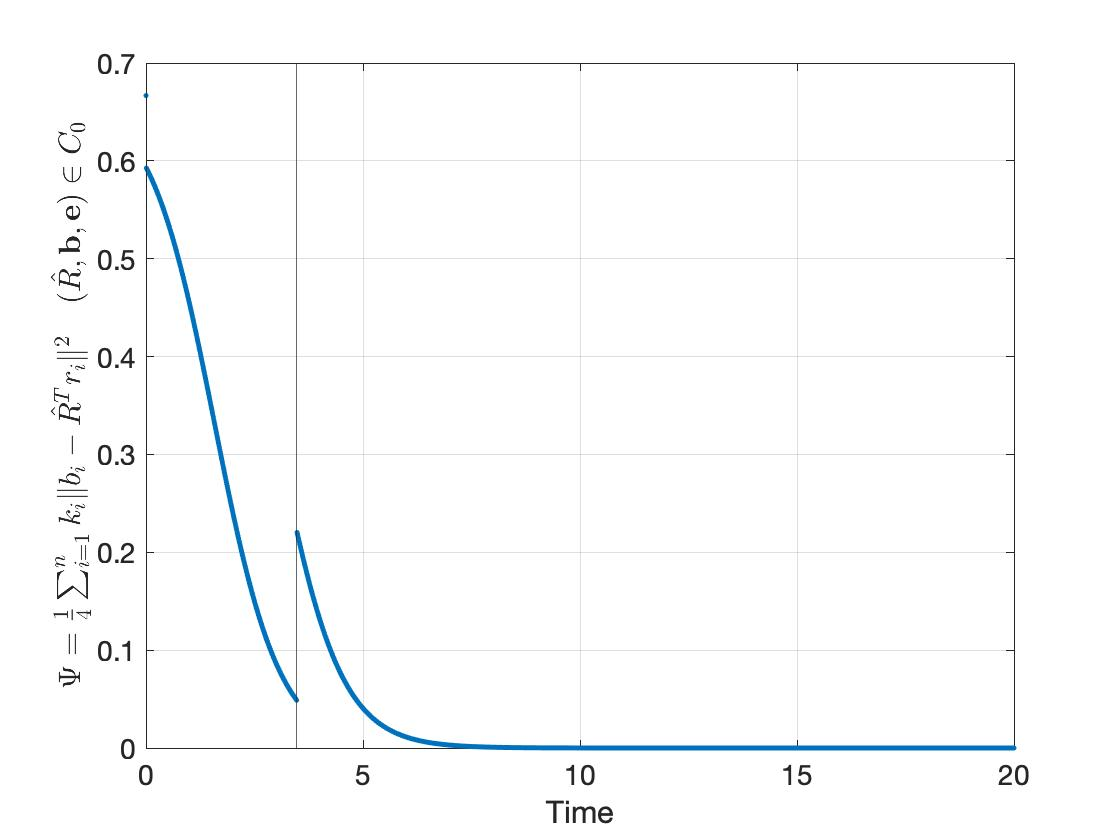
\includegraphics[width=\linewidth]{Figures/ECF_potential_ECF.jpg}
  \captionof{figure}{Plot of $\Psi$ vs time.  Jumps are seen at $t_{j1}=0$ sec and $t_{j2}=3.472$ sec. For $t$ such that $t_{j1}\leq t\leq j_{j_2}$, $\Psi = \Psi(\hat{R}, \mathbf{b}, \Rstar^\top \mathbf{r})$, otherwise $\Psi =\Psi(\hat{R},\mathbf{b}, \mathbf{r})$. This hybrid estimation error function is strictly decreasing during flows. }
  \label{fig:ECF_potential}
\end{minipage}\hfill
\begin{minipage}{.45\textwidth}
  \centering 
  \vspace{0pt}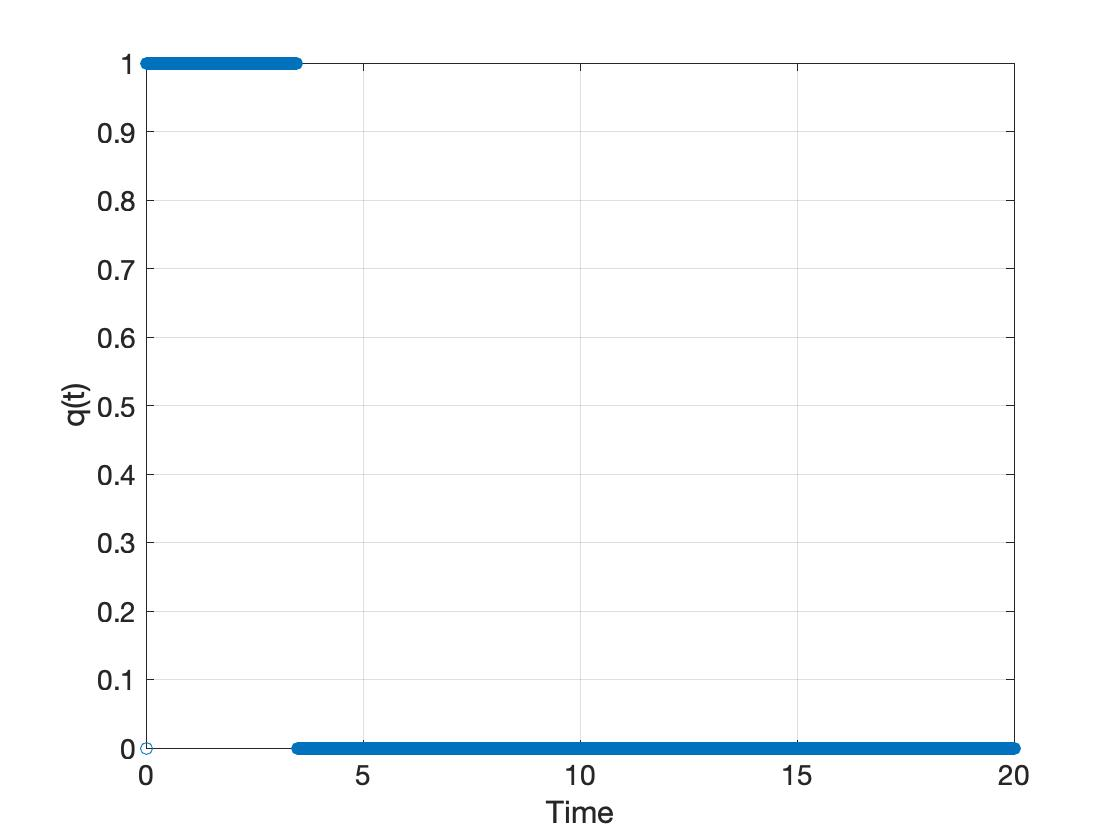
\includegraphics[width=\linewidth]{Figures/ECF_q.jpg}
  \captionof{figure}{Plot of $q(t)$ vs time. Jumps are seen at $t_{j1} = 0$ sec and at $t_{j2}=3.472$ sec. $q(0,0)=0$, after which a jump occurs since $\Psi(\hat{R}, \mathbf{b}, \mathbf{r})=1-\xi$.}
  \label{fig:ECF_q}
\end{minipage}
\end{figure}

\section{ECF with biased angular velocity measurements}
The measurement model used in \eqref{eq:hybridECF_ISS} did not consider bias in the angular velocity measurements that is inadvertently introduced by the gyroscope. Here, we consider the bias $\bias\in\R{3}$ in the angular velocity measurements, resulting in the following measurement model 

\begin{align}
    \Omegay = \Omega + \bias + \noisegyro && b_i = R^\top r_i + \eta_i, \quad i=1,...,n
\end{align}
where $\noisegyro\in\R{3}$ represents the noise in gyro measurements and $\eta_i, i=1,...,n$ represents the measurement noise in the vectorial direction measurements. Now, the bias is also estimated, and the estimate is denoted by $\biasHat$. Following \cite{mahony_complementaryFilter}, the hybrid explicit complementary filter with bias estimation is given below. Define $\omega_0 \coloneqq \omega_{mes}(\hat{R}, \mathbf{b}, \mathbf{r})$ and $\omega_1 \coloneqq \omega_{mes}(\hat{R}, \mathbf{b},\Rstar^\top \mathbf{r})$.

\bibliographystyle{plain}
\bibliography{ref}
\end{document}
